%%%%%%%%%%%%%%%%%%%%%%%%%%%%%%%%%%%%%%%%%
% Classic Lined Title Page 
% LaTeX Template
% Version 1.0 (27/12/12)
%
% This template has been downloaded from:
% http://www.LaTeXTemplates.com
%
% Original author:
% Peter Wilson (herries.press@earthlink.net)
%
% License:
% CC BY-NC-SA 3.0 (http://creativecommons.org/licenses/by-nc-sa/3.0/)
% 
% Instructions for using this template:
% This title page compiles as is. If you wish to include this title page in 
% another document, you will need to copy everything before 
% \begin{document} into the preamble of your document. The title page is
% then included using \titleAT within your document.
%
%%%%%%%%%%%%%%%%%%%%%%%%%%%%%%%%%%%%%%%%%

%----------------------------------------------------------------------------------------
%	PACKAGES AND OTHER DOCUMENT CONFIGURATIONS
%----------------------------------------------------------------------------------------



\documentclass[a4paper]{article}

\usepackage[utf8]{inputenc}
\usepackage{hyperref}
\usepackage{titlesec}
\usepackage{amssymb,amsmath}
\usepackage[italian]{babel}
\usepackage[titles]{tocloft}
\usepackage{appendix}
\hypersetup{%
    pdfborder = {0 0 0}
}
\usepackage{graphicx}
\usepackage[svgnames]{xcolor} % Required to specify font color
\usepackage{eurosym}

\newcommand*{\plogo}{\fbox{$\mathcal{PL}$}} % Generic publisher logo
\usepackage{listings}
\usepackage{fancyhdr}
\usepackage{lastpage}
\usepackage{ragged2e}

%----------------------------------------------------------------------------------------
%	TITLE PAGE
%----------------------------------------------------------------------------------------

\newcommand*{\titleAT}{\begingroup % Create the command for including the title page in the document
\newlength{\drop} % Command for generating a specific amount of whitespace
\drop=0.1\textheight % Define the command as 10% of the total text height

\rule{\textwidth}{1pt}\par % Thick horizontal line
\vspace{2pt}\vspace{-\baselineskip} % Whitespace between lines
\rule{\textwidth}{0.4pt}\par % Thin horizontal line

\vspace{\drop} % Whitespace between the top lines and title
\begin{center} % Center all text
\textcolor{Black}{ % Red font color
{\Huge Appunti}\\[0.5\baselineskip] % Title line 1
{\Large di}\\[0.75\baselineskip] % Title line 2
{\Huge Tecnologie Open Source}} % Title line 3
\\[2\baselineskip]
{\Large \version{}}

\vspace{0.25\drop} % Whitespace between the title and short horizontal line
\rule{1\textwidth}{0.4pt}\par % Short horizontal line under the title
\vspace{\drop} % Whitespace between the thin horizontal line and the author name

\end{center}
\vfill % Whitespace between the author name and publisher text
\vfill
{\large Luca De Franceschi}
\hfill
{\large Università degli studi di Padova}



%\rule{\textwidth}{0.4pt}\par % Thin horizontal line
%\vspace{2pt}\vspace{-\baselineskip} % Whitespace between lines
%\rule{\textwidth}{1pt}\par % Thick horizontal line

\endgroup}

\titleformat{\chapter}[display]
{}{\hfill\rule{.7\textwidth}{3pt}}{2pt}
{\hspace*{.3\textwidth}\huge\bfseries}[\addvspace{1pt}]
\titleformat{name=\chapter,numberless}[display]
{}{\hfill\rule{.7\textwidth}{3pt}}{2pt}
{\hspace*{.3\textwidth}\huge\bfseries}[\addvspace{1pt}]

\renewcommand*\contentsname{Indice}

\newcommand{\glossario}[1]{\textit{#1\ped{G}}}

\lstset{frame=shadowbox,
  aboveskip=3mm,
  belowskip=3mm,
  showstringspaces=false,
  columns=flexible,
  basicstyle={\small\ttfamily},
  numbers=none,
  numberstyle=\tiny\color{gray},
  keywordstyle=\color{blue},
  commentstyle=\color{dkgreen},
  stringstyle=\color{mauve},
  breaklines=true,
  breakatwhitespace=true
  tabsize=3
}

\renewcommand{\lstlistingname}{Listato}
\renewcommand{\footrulewidth}{0.4pt}

\newcommand{\changefont}{%
    \fontsize{5}{7}\selectfont
}


%----------------------------------------------------------------------------------------
%	CONSTANTS
%----------------------------------------------------------------------------------------

\newcommand{\version}{v0.9.0}

\newcommand{\authorName}{Luca De Franceschi}

%----------------------------------------------------------------------------------------
%	DOCUMENT HEADER
%----------------------------------------------------------------------------------------

\begin{document}
\justifying
\titleAT % This command includes the title page
\pagestyle{empty}
\newpage

\tableofcontents
\clearpage

%----------------------------------------------------------------------------------------
%	HEADER FORMAT
%----------------------------------------------------------------------------------------

\fancyhf{}
\fancyhead[RE]{\small\scshape\nouppercase{\leftmark}}
\fancyhead[LO]{\small\scshape\nouppercase{\rightmark}}
\fancyhead[LE,RO]{\small\thepage}
\lhead{\rightmark}
\rhead{\leftmark}
\rfoot{\thepage/\pageref{LastPage}}
\lfoot{\authorName}

\pagestyle{fancy}


%----------------------------------------------------------------------------------------
%	CONTENT
%----------------------------------------------------------------------------------------

\section{Introduzione}

Questo corso si divide fondamentalmente in due parti:

\begin{enumerate}

	\item Una prima parte \textbf{teorica} in cui si studierà il software libero, le licenze software, il progetto GNU, ...
	\item Una seconda parte \textbf{pratica} che si baserà su diverse tecnologie e in cui verrà enfatizzato l'aspetto pratico.

\end{enumerate}

\subsection{Informazioni tecniche}

Sito web del corso:

\begin{center}

\url{http://www.math.unipd.it/~tapparo/TOS/}

\end{center}

Indirizzo email del docente:

\begin{center}

\url{tapparo@math.unipd.it} [\textit{attivo solo durante il periodo del corso}]

\end{center}

Le lezioni si terranno in \textbf{Aula 1BC50}

Gli orari sono i seguenti:

\begin{itemize}

\item \textbf{Giovedì}, 9:30 - 12:05
\item \textbf{Venerdì}, 9:30 - 12:05

\end{itemize}

Il ricevimento avverrà durante gli intervalli, su appuntamento e dopo lezione.

\textbf{48 ore} di lezione, \textbf{6 CFU}, tutte lezioni frontali.

La modalità d'esame è solamente \textbf{orale}, e avviene tramite iscrizione su \textit{Uniweb}. Verterà in due parti: la prima parte è una discussione sugli argomenti affrontati a lezione, la seconda è una parte pratica sulle tecnologie libere affrontate lungo il corso.

\subsection{Programma del corso}

\begin{itemize}

\item Storia del software libero;
\item Licenze libere e caratteristiche del software libero;
\item Problemi aperti e prospettive del software libero;
\item Strumenti liberi di supporto allo sviluppo e alla cooperazione.

\end{itemize}

\subsection{Materiale}

Appunti delle lezioni. [\textbf{PRINCIPALE}]

Materiale nelle \textbf{slides}.

Molti libri di riferimento si possono trovare nelle slides. Molti sono reperibili liberamente.

Libri:

\begin{itemize}

\item \textbf{Open Source: strategie, organizzazione}, è il più accademico e viene toccato marginalmente dal corso. Offre buoni spunti per quanto riguarda la gestione manageriale del software;
\item \textbf{Il software libero in Italia}, un libro molto interessante composto da diversi interventi. Contiene una buona sezione riguardante le licenze;
\item \textbf{Hackers: Heroes of the Computers}, libro leggibile come un romanzo, molto consigliato, molto leggero ma va ben oltre gli obiettivi del corso;
\item \textbf{Software libero, pensiero libero}, per chi ha poca dimestichezza con il progetto GNU. Anche questo libro è composto da una serie di interventi. \textit{Stallman} ha una grande capacità di organizzazione degli argomenti;
\item \textbf{Free culture}, di \textit{Lawrence Lessig}. Quest'ultimo, oltre a essere l'ex leader di \textit{Creative Common}, ha scritto una serie di libri in cui affronta le tematiche di libertà di accesso ai \textbf{contenuti}. È un libro scritto molto bene, affronta il problema della rivisitazione dei modelli di proprietà a fronte di forti cambiamenti (es. l'introduzione di Internet, l'introduzione dei voli aerei...);
\item \textbf{Privilege and property}, accessibile da Internet. Viene affrontata la nascita del copyright.

\end{itemize}

\subsection{Note su questi appunti}
Gli appunti sono stati realizzati in LaTeX e sono il prodotto dell'unione degli appunti presi a lezione e la trascrizione delle registrazioni nell'A.A. 2013/2014. 

Il contenuto degli appunti potrebbe non coprire eventuali aspetti ed argomenti tenuti negli anni accademici successivi, Il registro utilizzato è simile a quello tenuto a lezione.

Il PDF ottenuto, eventuali stampe e altre opere derivate da questo sorgente sono da intendersi come rilasciate sotto licenza CC-BY-SA 4.0\url{https://creativecommons.org/licenses/by-sa/4.0/}


\subsection{Introduzione al software libero}

Il software libero non ha nulla a che vedere con il \textit{prezzo}, ma è un software che rispetta \textbf{4 concetti fondamentali}, ovvero 4 libertà per l'utente:

\begin{itemize}

\item Libertà di \textbf{usare} il software, usandolo senza restrizioni. Es. libertà di prendere il prodotto ed utilizzarlo senza limiti di tempo, senza vincoli di paese e per \textit{qualunque scopo} (didattico, lavorativo, privato, ...). Il tipo di utilizzo non è mai precluso. Questa è da un lato la libertà meno importante, ma dal punto di vista dell'impatto sull'utente sviluppatore non è la maggiore;
\item Libertà di \textbf{studiare} il software. A differenza del software proprietario è possibile vedere il \textit{codice sorgente} e capire come funziona il software, ciò da una garanzia di protezione all'individuo. Senza questa libertà si ha un blocco della conoscenza ed è una forte limitazione alla crescita del prodotto;
\item Libertà di \textbf{modifica}, ovvero posso prendere il software e cambiarlo, costruire nuove soluzioni. Il software libero è visto in questo contesto come \textit{piattaforma}. Si tratta di costruire delle proprie versioni a partire da una base. È una libertà molto importante ed è una ricchezza per poi creare altri sviluppi;
\item Libertà di \textbf{ridistribuzione}, in questo caso le aziende non solo possono creare per se stesse, ma anche mettere la nuova versione a disposizione di altri. Software libero come bene comune (\glossario{Routes}, \glossario{Beowulf}, \glossario{nslu2}). Una volta che posso ridistribuire ad altri allora il mio lavoro diventa realmente usabile. La redistribuzione abbatte i costi e aumenta l'apporto di contributi tramite la community che acquisice competenze e vsibilità al migliorare del software. Con un piccolo sforzo di molti si ottiene un grande risultato.

\end{itemize}

\subsection{Libero != Gratuito}

È un errore comune confondere questi due concetti, ma essi sono realmente due cose distinte. Esiste software gratuito ma che non è libero ed esiste software libero non gratuito (\textit{openerp}, i programmi della \glossario{fsf}, i binari \glossario{RedHat Enterprise Linux}). C'è tutta una serie di software \glossario{freeware} o \glossario{shareware} (es. \textit{winzip}). Un software shareware è collegato ad un acquisto successivo, invita l'utente ad acquistare una versione commerciale.

\glossario{\textbf{openerp}} è un software a pagamento che fornisce supporto e assistenza tecnica garantendo plugin e funzionalità aggiuntive. 
\glossario{\textbf{Free Software Foundation}} distribuisce software libero disponibile per diverse architetture. Ha una serie di programmi non facili da compilare. Si scarica il sorgente e si tenta di compilarlo, oppure si richiede il CD con i file già compilati, e questo CD viene fatto pagare.

\glossario{\textbf{RedHat Enterprise}} risolve bug e problemi nel minor tempo possibile e fa il porting di nuove funzioni su vecchie versioni. Vengono distribuiti i sorgenti ma non i binari. Molte di queste modifiche apportate da sviluppatori RedHat vengono integrate in \glossario{\textbf{CentOS}}

I concetti di \textbf{libero} e \textbf{gratuito} sono dunque concetti ortogonali.

\subsection{L'importanza del software libero}

L'importanza del software libero è legata in primo luogo alla \textbf{riduzione dei costi} (apache, php, ...). Non è importante per il pagamento in sé ma in quanto mobilita le leggi del mercato. È un mercato aperto, con un tasso più alto di competizione ed innovazione nel quale è facile entrare (ha basse tariffe d'ingresso) ed investire.

Un secondo impatto riguarda la \textbf{trasparenza}. Se quello che faccio è visibile, è anche controllabile da altri sviluppatori. È difficile fidarsi di un software che non si sa bene cosa faccia. Il software libero è una \textbf{garanzia} in quanto il controllo collettivo migliora la qualità del software.

Con il software libero non abbiamo nessun \textbf{lock-in}, il software libero si può adattare facilmente alle versioni precedenti e quindi non si creano dipendenze da software specifico (come nel caso di software proprietario come \textit{Microsoft Office}).

\textbf{Sicurezza e affidabilità?} Non ci sono dimostrazioni effettive che questo sia vero. Da un lato il software libero è visibile a tutti, ma dall'altro la manutenzione è costosa ed è facile introdurre bug. Il software proprietario vive molto spesso di un inflazione di \textit{features}, questo per aumentare le vendite.

%TODO (citazione di Bill Gates)

Si passa da un modello gerarchico produttore - consumatore in cui c'è [\textbf{chi fa}] ed ha il potere derivato dalla conoscenza e [\textbf{chi usa}], e sta alle condizioni. Il software libero è conoscenza libera. Si cambia il modo in cui si sviluppa e con cui si fa impero. È un modello ``\textit{social}'', il software vale molto di più per il fatto che c'è una \textbf{comunità} che gli gira intorno. Il rapporto che si viene a creare con gli utenti è molto importante (\textit{Innovation happens elsewhere}). Intorno al software libero si può creare una comunità in modo che la somma dei costi per fare un prodotto è minore rispetto al costo della comunità stessa.

\subsection{Introduzione a GPL}

Per molto tempo il software libero ha avuto una \textbf{posizione di inferiorità}. Le aziende prendevano software libero, sviluppavano una nuova versione e le rilasciavano come software proprietario. Il progetto \textbf{GNU} voleva creare una versione completamente libera del software. Ha creato dunque una nuova licenza, chiamata \textbf{GPL} (General Public License), in modo che avesse un \textit{effetto virale}. Una licenza libera ma con una restrizione particolare, ovvero ogni redistribuzione deve essere rilasciata sotto licenza GPL (circolo virtuoso e virale). Vedere il software libero come un'enorme libreria di conoscenza sempre disponibile.

Il software libero con questa licenza si arricchisce molto, cresce nel tempo e diventa sempre più interessante. Questa licenza è ancora molto presente (60\%, 70\% del software libero è sotto GPL).
\section{La nascita del copyright}

\subsection*{Materiale di riferimento}

\begin{itemize}

\item \textit{Privilege and Property Essays on the History of Copyright} - Ronan Deazley, OpenBook Publishers;
\item \url{http://digital-law-online.info/lpdi1.0/index.html} - sezione riguardo il copyright sul software;

\end{itemize}

\subsection{La storia}

Le prime forme di protezione in realtà non erano pensate per proteggere i diritti del beneficiario ma per dare dei vantaggi alle autorità che le emanavano; in secondo luogo non erano collegate alla conoscenza che raccoglieva quello si voleva proteggere, non si proteggeva il contenuto del libro ma si proteggeva l'ente industriale che lo aveva prodotto. Infine non erano collegate nemmeno all'autore. La forma era molto diversa da quella odierna.

Il copyright si è sviluppato in origine a Venezia intorno al 1469, 13 anni dopo la produzione della bibbia di Gutemberg. Prima dell'invenzione della stampa non c'era un sistema ben strutturato e organizzato, il libri costavano moltissimo, richiedeva anni di lavoro e di conseguenze non ve ne erano molti. Era un processo molto impegnativo la scrittura di un libro, stimato intorno agli 80.000 \euro{} di oggi. Nel 1450 la bibbia di Gutemberg cambia decisamente le carte in gioco, viene creato un processo industriale della scrittura, che prima era quasi un'``opera d'arte''. Lo stato incominciò ad interessarsene, per controllare il flusso di informazioni ed imporre dei blocchi sulla conoscenza; questa fu la direzione presa in Inghilterra. Dall'altro lato la stampa era un'invenzione fenomenale e si voleva trarre vantaggi da essa; questa fu la direzione presa a Venezia, i quali erano molto interessati ad avere il sistema di stampa e a sfruttarlo; cercarono di fare in modo che tanta gente ce l'avesse, imponendo comunque dei controlli. In quest'ottica il copyright non nasce come un diritto, ma come forma di privilegio che l'autorità concede, ha una forma di incentivo brevettuale.

In Italia esistevano delle \textbf{corporazioni}, che detenevano il controllo sulla conoscenza delle arti artigiane, vi era tutto un sistema di privilegi ed erano loro a mantenere l'ordine. Dall'altra parte gli stessi comuni che avevano creato queste corporazioni avevano anche creato un sistema per incentivare la gente degli altri comuni di svelare la conoscenza e diffondere le tecniche più avanzate. 

Quando nel 1469 Johannes of Speyer andò a Venezia chiese una forma di incentivo per portare la propria macchina di stampa a Venezia, e ovviamente glielo concessero, perchè era una macchina importante dalle grandi potenzialità. Gli diedero dunque un'esclusiva sulla stampa per 5 anni. Al giorno d'oggi quello che conta di un libro è il suo contenuto, non la forma; all'epoca si pagavano i libri in funzione del peso o come merce di scambio. Pochi mesi dopo questa esclusiva però Johannes morì, e questo privilegio durò dunque per pochi mesi, e preso si cominciò dunque a formare un mercato sulla stampa. 

Una cosa importante che fu conseguenza di questo privilegio fu che il controllo della stampa venne sottratto alle corporazioni, la produzione si orientò dunque in un certo modo, non ci fu la differenziazione del modo in cui venivano gestiti i privilegi di stampa. Questi privilegi erano concessi volta per volta alle singole persone ed erano associati al modo in cui venivano prodotti i libri:

\begin{itemize}

\item Privilegi e non diritti d'autore; 
\item Era lo stampatore ad avere i diritti;
\item Carattere tecnologiche dei privilegi iniziali, non associati al contenuto.

\end{itemize}

Le opere all'epoca erano per la maggior parte diverse edizioni delle opere classiche.

Uno \textbf{statuto} importantissimo, quello del 1474, per la prima volta stabiliva che quando una persona produceva qualche cosa di meritevole, di nuovo e originale, aveva diritto ad una protezione per 10 anni. Questa sembra per la prima volta una forma di protezione collegata alla proprietà intellettuale di quello che ci sta dentro e non esclusivamente ad un processo industriale. Era una cosa che si avvicinava a un \textit{diritto}. Ma di fatto questo statuto finì in un binario morto ma ebbe un effetto molto importante, perchè si spostò l'attenzione per la prima volta dall'interesse degli stampatori agli \textbf{autori}. 

Il 1517 segna un cambiamento nel modo con cui vengono distribuiti i privilegi. Prima i privilegi venivano distribuiti in modo indipendente dal contenuto, quello che interessava era esclusivamente il processo di stampa. A un certo punto quando ci si stanca di avere tutti libri uguali della stessa opera, volevano avere libri un po' più \textit{nuovi}, e quindi ritirarono tutti i privilegi sui libri in stampa e le opere cadono nel pubblico dominio. Fu necessario dunque lo spostamento del mercato verso le opere originali, le quali erano proteggibili. Per una volta quello che conta non è il modo in cui viene stampato un libro ma quello che ci sta dentro. Gli \textbf{autori} cominciarono ad avere dunque un po' più di potere. Questa protezione sulle opere si rafforzò nel tempo, andando a proteggere anche le \textbf{modifiche} sulle opere. Come conseguenza di questo i privilegi cominciarono ad essere garantiti anche agli autori.  

La regolamentazione delle arti artigiane era fatta dalle corporazioni, ma piano piano sempre più persone le stavano trovando più adatte. Si stava entrando nel rinascimento, un'epoca in cui si da più spazio all'uomo e alla sua creatività. Le corporazioni avevano il compito di regolamentare le arti, di proteggerle; ogni comune aveva le proprie. Una conseguenza importante di ciò fu la nascita del concetto di ``\textbf{proprietà immateriale}''. Si aveva la netta sensazione che quello che una persona conosceva era importante. D'altra parte la forma di protezione era strettamente legata alla comunità e la comunità va protetta proteggendo l'informazione. Questa forma di privilegio era molto legata agli autori e non più ai produttori. Si spostò l'interesse dal processo di produzione del libro al suo contenuto e in particolare all'autore.

Il sistema brevettuale parallelamente collegò il concetto di proprietà immateriale alla persona, anche perchè questo è un periodo in cui c'è uno spostamento generale dalla comunità alla persona (umanesimo). Questo ebbe un grosso impatto. Prima chi gestiva la conoscenza erano degli artigiani, con la nascita di un interesse culturale diventa più ``teorico'', nasce una differenza tra la proprietà intellettuale e i suoi prodotti. Questo venne rafforzato ulteriormente dalla nascita degli \textbf{scrittori di professioni}. Il valore delle opere deriva dall'individuo e dalle sue conoscenze.

Nel 1600 in Inghilterra si era sviluppata tutta una vita politica pubblica, in cui si discuteva pubblicamente e ci si formava un'opinione, per esempio nei vari caffè. A un certo punto si sentì il bisogno di controllare questa opinione pubblica; prima esisteva una struttura chiamata \textit{camera stellata} che era un tribunale ``fittizio'', una forma di censura che permetteva di controllare ciò che veniva espresso dalla gente. Nel 1641 venne abolita e a quel punto ci fu la necessità di sostituire questa forma censoria. Questi controlli vengono implementati nel 1643/1644, in ci ci fu un rigido controllo pre-stampa e la censura fu affidata alla \textbf{stationer's company}, alla quale era affidato il compito di decidere chi poteva stampare. Naturalmente il diritto lo aveva solo chi si dimostrava premuroso nei confronti dei diritti della corona. Questa legge venne prorogata diverse volte fino al 1695. 
\section{Storia del software libero}

\subsection{Gli albori}

1950 - 1960, la cultura hacker nasce ai laboratori del \textbf{MIT}. Nel 58/59 nascono i primi corsi di \textbf{intelligenza artificiale} (di fatto era informatica). Vi era un rapporto \textit{giocoso} tra il gruppo di ricerca e i ragazzi, un rapporto che funzionava molto bene. Il primo gruppo hacker nasce come sottogruppo di \glossario{S\&P}. All'inizio non era una vera e propria comunità hacker ma c'era solamente un gruppo che frequentava i corsi e morta lì. L'accesso ai PC all'epoca era molto riservato (ai docenti, al personale). Questo gruppo aveva trovato una sala (407) con delle macchine perforatrici (per programmare le schede perforate). 

Il rapporto cambierà con l'evoluzione delle tecnologie, con l'accesso più libero alle nuove macchine (ATX0). Con il cambiamento delle tecnologie cambia anche la gestione (si poteva accedere liberamente alle macchine), si cominciò a formare un gruppo di persone che \textit{bazzicavano} sulle macchine. Si formò così una comunità con idee e un'etica in comune. 

Con il \glossario{PDP} (computer) le cose cambiarono ulteriormente. IL PDP era pensato non per il \textit{best-processing} ma per una computazione interattiva (aveva un monitor ...), costava inoltre molto meno ed era quindi più accessibile. A quel punto diventava possibile utilizzare le macchine a costo zero.

\subsection{Etica hacker}

L'etica che si sviluppò all'interno della comunità si basava sui seguenti 4 punti:

\begin{enumerate}

\item \textbf{Libero accesso all'informazione}, bisogna poter metterci le mani, e questo non era all'epoca garantito a tutti;
\item \textbf{Decentralizzazione}, potere che si sposta dal centro;
\item Gli hacker dovrebbero essere \textbf{giudicati solo per il loro valore};
\item Il software come \textbf{espressione artistica}, va oltre quello che è la pura utilità, va a fare qualcosa che è divertente e bello (creazione di giochi). Doveva essere un piacere che andasse agli altri;

\end{enumerate}

\subsection{Conseguenze dello sviluppo software}

In questo momento c'è una libera condivisione del codice, non esiste software protetto da copyright. Non c'era interesse nel proteggerlo. Il software era un'appendice dell'hardware. Le macchine erano in continua evoluzione e modifica. L'avere un accesso a come il software funzionava era vitale per gli sviluppatori. Dato che il tempo macchina era oneroso, bisognava sfruttarlo al meglio e quindi era importante la condivisione del lavoro tra gli sviluppatori.

\textbf{Incopatible Time Sharing}, ci si compra un terminale e poi si accede alle reti di calcolo di un enorme computer. ITS era la base di questo concetto. Non c'erano password, ogni utente aveva i propri file personali accedibili da tutti. Era disegnato per la cooperazione tra gli hacker ed assumeva una grossa fiducia negli utenti.

\subsection{La fine del periodo degli hacker}

\begin{itemize}

\item 68: il computer lab viene isolato;
\item 70's-80's: frammentazione della cultura hacker:

	\begin{itemize}

	\item 1976: copyright act;
	\item \glossario{Symbolics} recluta la maggior parte degli hacker rimasti al MIT;
	\item Altri hacker fondano \glossario{LMI}.

	\end{itemize}

\item Negli '80 cessa la produzione del PDP-10, condannando definitivamente ITS.

\end{itemize}

\subsection{Nasce unix}

Una serie di circostanze ha voluto che \glossario{unix} venisse rilasciato con licenza libera (era comunque protetto da copyright). Nasce come una risposta a \glossario{MUTIX} per creare un sistema diverso, più piccolo e con minor risorse. Fu il primo sistema scritto non direttamente in linguaggio macchina ma scritto in linguaggio C. Questo sistema ebbe subito un grosso successo anche e soprattutto in ambito universitario. 

L'\glossario{AT\&T} era un monopolio telefonico del governo, aveva la restrizione che non poteva vendere software e quindi si decise di distribuire gratuitamente unix. Al suo lancio esso si diffuse molto rapidamente. Una delle università che lo utilizzò fin da subito fu \textbf{Berkeley}, che aveva interesse dal punto di vista della programmazione interna di unix. Nel 1977 nacque \glossario{BSD}, una versione modificata di unix utilizzata dall'università. Due anni dopo la AT\&T annunciò di voler commercializzare unix. 

Nel 1983 AT\&T viene divisa e unix diventa commerciale. A questo punto c'era BSD ed era una possibile scelta. \glossario{ARPA} lo utilizzò per creare \glossario{ARPANET}, per collegare diversi computer via network, garantendo un'uniformità a livello software del sistema operativo. Il software libero ebbe quindi un impatto notevole. ARPA mise inoltre a disposizione dei fondi per migliorare BSD e facilitare il suo sviluppo. In seguito venne citata in giudizio dalla AT\&T perchè si diceva volesse il codice di unix. Questo bloccò di fatto lo sviluppo di ARPANET. Se ciò non fosse successo probabilmente non sarebbe nato unix.

\subsection{Nasce il progetto GNU}


\section{L'ultimo degli Hacker}

Analizziamo la fase di decadenza degli hacker, qui entra in gioco Richard Stallman.

\subsection{Bibliografia}

\begin{itemize}

\item Steven Levy: \textit{Heroes of the computer revolution};
\item Sam Williams: \textit{Free as in Freedom (2.0): Richard Stallman and the free software revolution}

\end{itemize}

\subsection{Prime esperienze}

Richard Stallman nasce a New York nel 1953 dove si forma dal punto di vista informatico, diventa un esperto di \glossario{Assembler}, di sistemi operativi e di editor di testo. Inizia con le prime esperienze nel centro scientifico di Manhattan, poi lo assumono e inizia a sviluppare programmi in Fortran per il calcolo numerico. Nel 1971 entra ad Harvard e si laurea in Fisica. Scopre in segreto un'affinità con la cultura hacker sviluppatasi al MIT. Venne notato da Russ Noftsker e in seguito assunto al MIT come programmatore di sistemi. Viene preso sotto l'ala protettiva di Richard Greenblatt e Bill Gosper, che gli fanno da mentore.

\begin{figure}[htbp]
\centering

\includegraphics[width=50mm]{images/stallman.jpg}
\caption{Richard Stallmann da giovane}
\end{figure}

\subsection{Emacs}

Una delle prime cose che Stallman fece fu la creazione di \glossario{Emacs}. Inizialmente esso era pensato come un insieme di macro per \glossario{TECO}, utlilizzato da tutti, che era una sorta di linguaggio per scrivere e non era assolutamente real-time. Creò dunque una sorta di editor dentro TECO. Guy Steele ebbe in seguito l'idea di fare un po' di ordine tra le macro (che erano diventate tantissime). Quest'opera fu continuata da Stallman, in modo da avere un insieme più omogeneo. Questo disordine non sarebbe dovuto replicarsi in futuro, bisognava evitare che ciascuno costruisse il proprio insieme di macro. Stallman voleva fare qualcosa di ``sociale'', voleva andare un po' oltre e impedire ulteriori disordini. Quindi si imposero delle restrizioni sulle modifiche delle macro. Questa condizione creò una sorta di comunità in cui i programmatori condividevano gli sforzi di programmazione ed evitavano la dispersione del lavoro. Questo fu il primo gruppo concreto di condivisione del software e il primo mattone della nascita della GPL. Emacs è nato in questo modo, ma poi è stato ritradotto varie volte.

\begin{figure}[htbp]
\centering

\includegraphics[width=20mm]{images/emacs.png}
\caption{Il logo di emacs}
\end{figure}

\subsection{Le prime incursioni}

Allo stesso tempo si iniziarono a vedere le prime debolezze. Il dipartimento di difesa obbligò gli hackers a programmare sui sistemi del dipartimento di \textit{computer science} del MIT, in cui c'era mancanza di accesso libero all'informazione. Arrivarono al punto di fare una sorta di ``sciopero'' nei confronto del laboratorio e bloccarono l'accesso alle succesive versioni di Emacs. Si creò dunque una frattura tra Richard Stallman e la comunità.

Gli hackers cominciarono a migrare e andarono a lavorare altrove per altre società. Comparirono i primi programmi coperti da copyright nel campo dell'\textbf{intelligenza artificiale}.

\subsection{La lisp machine e il collasso}

Richard Greenblatt, un programmatore del MIT, era un'autorità nel settore. Aveva iniziato a giocare con le \glossario{lisp machine} (lisp era un linguaggio ad alto livello) e aveva avuto l'idea di creare una macchina che eseguisse lisp in modo più efficiente e sicuro. Creò una sorta di controllo all'interno di lisp per la gestione delle risorse, aveva modificato la struttura dell'hardware in modo che lisp venisse utilizzato più velocemente. Questo fu un grosso passo avanti, perchè programmare in lisp era molto più comodo che programmare in assembler. Alla lunga riuscì ad ottenere lo stanziamento di fondi per 6 macchine. Si arrivò a produrne 32. Anche per gli hacker era un mondo nuovo, perchè cambiava la visione classica (un solo computer disponibile), ora ogni persona aveva la propria macchina. Pensò dunque di collegare queste 32 macchine per favorire la condivisione. Il progetto è cresciuto a un punto tale che si trasformò in un azienda per la produzione di lisp machine, che in un certo senso era un'estensione del MIT. La visione di Greenblatt era quella di un'azienda \textit{``hacker friendly''}. Russel Noftsker non condivideva molto l'idea, era parte del progetto, ma la sua visione era incompatibile con quella di Greenblatt, pensava che l'azienda non sarebbe stata in grado di produrre grosse modifiche a livello globale.
Nel 1979 si arriva al punto in cui il conflitto esplode (Greenblatt aveva dalla sua un caratteraccio, non teneva conto delle persone). Da un lato non si poteva ``far fuori Greenblatt'', ma dall'altro non c'erano molte persone che volessero continuare con la sua visione (Greenblatt voleva avere l'ultima parola), quindi in sostanza non esisteva un team. Perciò gli diedero un anno di tempo per fondare l'azienda, altrimenti gli altri avrebbero fondato la loro. Riuscì sorprendentemente a creare un'azienda che funzionasse, la \glossario{LMI}, ma dopo un anno gli altri suoi colleghi crearono \glossario{Symbolics}.

\begin{figure}[htbp]
\centering
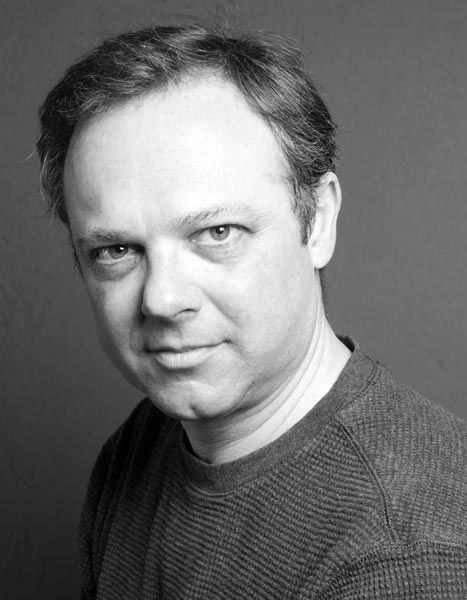
\includegraphics[width=50mm]{images/greenblatt.jpg}
\caption{Richard Greenblatt da giovane}
\end{figure}

\subsection{Lo svuotamento del MIT}

LMI e Symbolics attingono pesantemente dal MIT (concorrenza). Nel 1982 Symbolics rende le proprie modifiche al sistema operativo delle lisp machines proprietario. A questo punto c'è un crollo della comunità, era già molto debole, erano rimasti pochi hackers ma c'era comunque un sistema complesso che andava mantenuto. 
Quindi a un certo punto PDP divenne obsoleto e la comunità si ritrovò di fronte a un problema, bisognava creare una nuova macchina, era necessario prendere tutto il software delle macchine correnti e riscriverlo, e gli hackers non erano abbastanza numerosi. Alla fine si decise di comprare il sistema operativo proprietario di \glossario{Digital} e a partire da esso si creò \glossario{Twenex}, con caratteristiche molto diverse da un sistema standard (sicurezza costruita nel sistema). 
Il gruppo wheel era un gruppo i cui programmatori erano gli unici che potevano divenire amministratori e apportare modifiche alla macchina. In seguito ci fu la nascita di GNU.

\subsection{L'appello}

nel 1983 Richard Stallman fece un appello su \texttt{net.unix-wizards}:

\begin{center}

\textit{``Starting this Thanksgiving I am going to write a complete Unix-compatible software system called GNU (for Gnu’s Not Unix), and give it away free to everyone who can use it. Contributions of time, money, programs and equipment are greatly needed''}.

\end{center}

Le ragioni della scelta di unix furono:

\begin{itemize}

\item Il monopolio della AT\&T;
\item La familiarità con il codice sorgente (e grosso utilizzo da parte delle università), c'era un grande numero di utilizzatori e di sviluppatori;
\item La portabilità (sviluppato in C e non in assembler), sistema che si adattasse alle macchine, su architetture molto diverse.

\end{itemize}

\subsection{GNU Emacs}

La prima cosa che serviva era un programma per eseguire il codice, quindi ci fu un grosso lavoro sul compilatore. Stallman parte dal codice di Gosling e scrive GNU Emacs. L'Emacs del MIT non andava bene, serviva una nuova versione che andasse bene per le macchine piccole. Si erano nel frattempo creati tutta una serie di \textit{cloni} di Emacs, una di quelle era scritta da James Gosling e quest'ultimo concedette a Stallman il codice senza problemi, dal quale potè creare una nuova versione.
Unipress a quel punto minacciò legalmente Emacs (aveva acquistato la versione di Gosling), ma per fortuna di Stallman la versione era stata riscritta praticamente da zero, per cui non ebbe problemi e nel 1985 rilasciò ufficialmente il programma. 
\linebreak
\linebreak
Stallman decise di pensare bene a una licenza per la versione, basandosi su GNU. La licenza era basata principalmente sulla licenza implicita della comunità Emacs. È il primo grosso progetto di GNU, che sotto sotto era una GPL. A partire da esso si svilupparono tutta un'altra serie di progetti, bisognava creare dunque una licenza che fosse comune a tutti. Gilmore suggerì dunque il cambio di nome e nacque la GNU general public license che venne distribuita in versione 1.0 con il rilascio di \glossario{gdb}.

\subsection{L'incontro con BSD}

AT\&T cominciò a focalizzarsi sull'utilizzo di Unix a scopo commerciale e nel frattempo si sviluppò BDS, una distribuzione di Unix derivata con scopi accademici e con diversi contributi esterni. L'idea era di trasformare i loro sistemi operativi \textit{batch} con una versione di Unix.
Due studenti si erano appassionati e avevano reso una versione migliore di BSD, aggiungendo tutta una serie di cose, iniziando dapprima a effettuare modifiche esterne e poi interne. Quindi si formò una distribuzione indipendente, ma c'era la necessità della licenza AT\&T. Stallman convinse Bostic e i suoi a creare una versione completamente libera (all'inizio era un po' deficitaria ma col tempo si è messa in pari). A questo punto c'era un sistema operativo (e un kernel) libero.

\subsection{Anni 80-90}

Intorno alla costellazione GNU ci furono vari programmatori che iniziarono a rilasciare codice sotto licenza GPL. Bruce Perens rilascia \textit{electric fence} sotto licenza GPL, una libreria per le chiamate all'allocazione di memoria. Bruce Perens sarebbe diventato in seguito il project leader di Debian.
\linebreak
\linebreak
GPL stava dunque divenendo una licenza molto importante. Rich Marin fonda \glossario{Prime Time Freeware}, un'azienda che rilascia software solo sotto GPL. L'azienda \glossario{Cygnus} con Micheal Tiemann aveva cominciato a lavorare al progetto \glossario{gcc}, aggiungendo il supporto al C++. Il progetto era quella di contribuire (fare modifiche) al gcc e poi rivenderlo. L'idea ebbe un notevole successo. Cygnus venne fondata nel 1990 e per la fine dell'anno valeva 725000\$ in supporto e contratti.

\subsection{Espansione del progetto GNU}

Il progetto GNU si espanse in modo molto rapido e virale. Di seguito vengono riportati i maggiori rilasci dei primi anni:

\begin{itemize}

\item gcc;
\item Libc (1987);
\item Bash (la shell), fileutils (gestione dei file), sh-utils, textutils (gestione dei testi);
\item Ghostscript;
\item Textinfo (formattazione della documentazione, l'html lo renderà obsoleto);
\item Yakk, make, ...

\end{itemize}

\subsection{GNU Hurd}

Quello che mancava era un kernel, ed era molto complesso svilupparlo. All'inizio le macchine disponevano di un sistema unix proprietario. Vi era dunque la necessità di creare un \textbf{kernel libero}. Nel 1986 ci fu il primo tentativo di basare il kernel su TRIX, ma oltre a non funzionare sulle macchine standard richiedeva troppi cambiamenti. In seguito si sviluppò l'idea di basarsi su BSD, ma c'era poca collaborazione da parte degli sviluppatori bsd, si preferisce un approccio più ambizioso.
Svilupparono dunque un micro-kernel basato su \textbf{Mach}, ma inizialmente non era libero e dovettero aspettare che ``\textit{venisse liberato}''. Nel 1990 iniziarono dunque i lavori sul kernel, ma ci furono diverse difficoltà nello sviluppo. Poi arrivò \textbf{linux} e dunque molti sviluppatori posarono ad esso la loro attenzione. Allo stato attuale ci sono stati tutta una serie di progressi:

\begin{itemize}

	\item Driver linux disponibili via DDE;
	\item Supportato X, iceweasel, ...;
	\item Porting di debian.

\end{itemize} 
\section{Il movimento open-source}

\subsection{Materiale di riferimento}

\begin{itemize}

\item \textit{The Daemon, the GNU and the Penguin: a history of Free and Open Source} - Peter Salus;\\
Capitoli 9, 18, 19, 20, 22 \\
Disponibile sotto Creative Common all'indirizzo: \\
\url{http://www.debian.org/doc/manuals/project-history/}
\item \textit{Breve storia di Debian} - disponibile all'url:\\
 \url{http://www.debian.org/doc/manuals/project-history/}.
\item \textit{Lions' Commentary on UNIX 6th Edition, with Source Code}\\ \url{http://v6.cuzuco.com/}

\end{itemize}

\subsection{MINIX}

Unix era un sistema operativo vero e proprio, ed era molto complesso. John Lions, un famoso sviluppatore Australiano, pubblica il codice sorgente commentato di UNIX in un'opera storica denominata: \textbf{Lions' Commentary on UNIX 6th Edition, with Source Code}. Ma con l'avvento della versione 7 di unix vengono imposti tutta una serie di blocchi: l'opera di Lyons viene bloccata, aumentano i costi delle licenze e vi sono delle restrizioni sull'insegnamento in classe. Molte università interruppero dunque l'insegnamento di unix; questo fu un cambiamento abbastanza stupido, perchè ciò che aveva reso forte unix era la diffusione nel mondo accademico. 

Andrew S. Tanenbaum era all'epoca un insegnante di \textit{computer science} e venne molto toccato da questa decisione, in quanto aveva sempre insegnato basandosi su unix. Decise allora di creare \textbf{MINIX}, un sistema operativo abbastanza importante, minimale, per scopi didattici, pensato per essere \textbf{semplice}. Era un sistema a micro kernel, rilasciato sotto \textbf{licenza permissiva} ma non libera. Aveva inoltre scritto un libro che documentava e spiegava MINIX. Ma questo sistema operativo aveva una grossa limitazione: \textbf{mancava un emulatore di terminale}.

\subsection{Linux}

Linus Torvalds è stato uno dei primi utilizzatori di MINIX. Nasce ad Helsinki nel 1969. Nel 1990 frequenta l'Università di Helsinki, comincia a studiare Tanenbaum e comincia a fare le prime modifiche per provare a creare un emulatore di terminale. Nel 1991 Lars Wirzenius (un amico di Torvalds) lo porta alla conferenza di Stallman, nella quale ebbe una prima esposizione al progetto GNU. Il 5 Gennaio 1991 Torvalds:

\begin{itemize}

\item Compra un PC (un 80386);
\item Ci installa MINIX;
\item Inizia a scriverci un emulatore di terminale (scritto in C e in assembly).

\end{itemize}

\begin{figure}[htbp]
\centering
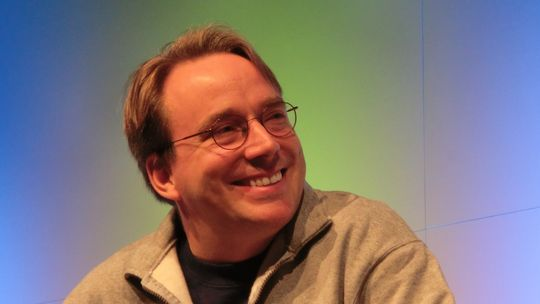
\includegraphics[width=50mm]{images/linus-torvalds.jpg}
\caption{Linus Torvalds}
\end{figure}

La prima versione di \textbf{Linux} è la A e la B, fatta solamente da due finestre. Da emulatore di terminale com'era pensato in origine Linux d lì il è stato espanso fino a crearci un vero e proprio sistema operativo \textbf{Linux 0.0.1} con un kernel funzionante.

Già nel 1992 il sistema era diventato molto importante. Torvalds decide dunque di rendere il sistema \textbf{indipendente} da MINIX (ci fu anche una disputa con Tanenbaum). Cambiò dunque la licenza adottando la GPL, che considerava buona per il suo sistema operativo, a prescindere dal software GNU stesso. Nascono inoltre già le prime distribuzioni basate su linux, come ad esempio SUSE, MCC o la prima distribuzione commerciale: LGX. Queste distribuzioni rendevano decisamente più facile l'utilizzo di Linux (di per sè molto complesso).

Nel 1994 viene rilasciato \textbf{Linux 1.0} e fu lo stesso Torvalds a presentarlo in una conferenza tenutasi ad Helsinki. Già allora era un sistema utilizzabile.

Ancora nel 1993 erano nate le prime versioni commerciali: Bolzern, Flagship e \textbf{Linux Pro}. Nel 1994 nasce inoltre \textbf{RedHat}, creato da Marc Ewing, e diventa ben presto la più diffusa distribuzione Linux.

Nel 1996 fu scelto come logo ufficiale di Linux un pinguino disegnato da Larry Ewing, chiamato \textbf{Tux}, come abbreviazione di \textbf{T}orvalds \textbf{U}nix.

Sempre nel 1996 esce \textbf{Linux 2.0} con supporto a microprocessore. Con la versione 3.0, uscita nel 2011, le modifiche sono state molto più incrementali. Nel corso degli anni con la 2.0 il grado di utenza era ancora molto piccolo.

\begin{table}[htpd]
\centering
	\begin{tabular}[c]{l | l | l}
	\hline
	& 1992 & 2012 \\
	\hline
	Sviluppatori Linux & 100 & 1000 \\
	\hline
	Linee di codice Linux & 250.000 & 14.000.000 \\
	\hline
	\end{tabular}
\caption{Sviluppo di Linux negli anni}
\end{table}

Una volta c'erano molti sviluppatori \textit{volontari}, ad oggi il supporto è dato da grosse aziende che possono investire tempo e denaro su Linux.

\subsection{Debian}

C'era un forte legame tra il mondo degli hackers e il mondo del software libero. Si venne a creare una \textbf{nuova generazione di sviluppatori}. Volevano provare a costruire una distribuzione che fosse fortemente legata a certi principi, che mettesse insieme varie cose, che facesse da collante. A quel punto nacque \textbf{Debian}. Linux da un lato stava procedendo e crescendo velocemente ed aveva molte caratteristiche interessanti, ma dall'altro c'era una lontananza dai principi del software libero e dalla GNU. Questo era percepito come un problema da parte di una fetta della comunità. Ad altri invece la cosa andava più che bene, dunque si venne a creare una \textbf{divergenza}. 

Il progetto Debian venne fondato da Ian Murdock nel 1993, con l'intento di fare una distribuzione di Linux \textbf{completamente libera}. Entrò a far parte del progetto GNU nel 1994-1995. Nel 1994 venne redatto il \textbf{manifesto debian}, nel quale si riassumeva il significato e la filosofia di debian. La prima versione stabile (Debian 1.1 ``Buzz'') venne rilasciata nel 1996. Il project leader della Debian divenne Bruce Perens

La caratteristica principale di Debian è che pone l'attenzione in modo quasi maniacale alla qualità del software (a volte perdendo anche molto tempo) e al fatto che il software sia libero (solo software DFSG. Si basa su una \textbf{forte comunità} che gestisce (tramite votazioni) tutte le decisioni sullo sviluppo; chiunque può proporre cambiamenti e ognuno è responsabile delle proprie azioni (attenzione alla sicurezza). Un altro cardine su cui puntano gli sviluppatori Debian è una strenua \textbf{disponibilità} del software.

Debian è caratterizzato da un suddivisione (politica) in più parti del repository. Le uniche componenti che sono della Debian sono quelle libere e quelle che dipendono da software libero. Il software che è all'interno della Debian entra nell'archivio principale, \textbf{FREE}. Poi all'interno ci sono altre componenti ospitate nel server della Debian ma che non sono della Debian, \textbf{NON-FREE} che non aderisce alle \textit{DFSG}, \textbf{CONTRIB} (che è libero ma dipende da componenti non libere).

C'è una versione di Debian \textbf{stabile} (software un po' vecchio però), quella che ha superato tutti i bugfix, una versione \textbf{non stabile} e una versione \textbf{testing}. Nella versione non stabile ``\textit{può esplodere tutto da un momento all'altro}'', viene aggiornata ogni giorno. La testing entra nel pacchetto solamente se nell'ultimo mese non sono stati segnalati bug importanti.

Da un lato Debian ha molto software e dall'altro non avendo interessi commerciali, non ha interessi nel penalizzare la concorrenza. È gestita essenzialmente da volontari.

\subsection{La cattedrale e il bazaar}

Un altro personaggio molto importante nel mondo del software libero è Eric Steven Raymond, informatico e programmatore statunitense di grande esperienza, che nel 1997 pubblica ``\textbf{La cattedrale e il bazaar}'', un saggio sullo sviluppo del software. Esso era essenzialmente destinato ad affrontare il problema del perchè Linux, con il suo kernel, funzionasse così bene. Non era scontato che Linux funzionasse, anzi all'inizio, secondo la sua opinione, era destinato a ``scoppiare''. Il problema è che ognuno tendeva a pensare con la propria testa; eppure la cosa non succedeva. Quindi iniziò ad analizzare il fenomeno. 

Una delle prime cose che ha fatto è stato quello di iniziare un progetto, chiamato \textbf{popclient}, per l'invio e la ricezione della posta. Comincia dunque ad utilizzare tutta una serie di principi per la gestione di questo progetto per vedere se riusciva a ricreare il successo che aveva visto con Linux, un progetto che funzionasse bene e avesse una solida base di sviluppatori. Uno dei principi che aveva adottato era di trattare gli utenti come una sorta di \textbf{co-sviluppatori}, come se il programma fosse stato fatto insieme a loro. La comunità popclient divenne dunque molto attiva. 

Il secondo principio su cui basò il proprio lavoro fu: ``Distribuisci presto, distribuisci spesso e presta ascolto agli utenti'', in questo modo si favorisce la risoluzione di bachi in tempi brevi. Molti utenti si facevano avanti e miglioravano il software, sentendosi parte attiva del progetto. L'idea che secondo Raymond aveva fatto il successo di Linux era trasformare il software da uno sviluppo di una persona che ``dona agli altri'' a uno sviluppo ``social'', attorno al quale ruotava una comunità. Spesso la varietà delle persone porta ad una varietà di modi per risolvere il problema, vi sono approcci diversi, e la combinazione dei contributi può significare grossi miglioramenti.

L'articolo di Raymond ebbe una grossissima fortuna, l'impatto all'interno della comunità fu molto sentito, e l'effetto di questo fu che l'attenzione andò oltre la semplice comunità degli appassionati. Una delle conseguenze di questo successo fu che nel 1998 Netscape annunciò di voler rilasciare il codice sorgente del proprio browser, e disse che per decidere questo si era basato anche sull'articolo di Raymond. Una volta Netscape era dominante, prima dell'arrivo del colosso Microsoft con Internet Explorer. Il browser di casa Microsoft è sicuramente disprezzato al giorno d'oggi, ma in realtà per gli standard di allora era molto buono e la Microsoft era riuscita, partendo da zero, a recuperare terreno in tempi notevoli su Netscape. A Netscape non interessava moltissimo del suo navigatore, non poteva infatti guadagnarci (era gratis), ma focalizzava la sua attenzione sul mondo Server. Temeva però che se Internet Explorer fosse divenuto dominante a quel punto i propri server sarebbero stati ``scartati'' in favore di quelli di Microsft. Avrebbe perso una grossa fetta di mercato e buona parte del loro reddito. Ebbero dunque l'idea di rilasciare il codice sorgente di Netscape sotto una licenza libera. In questa decisione aveva avuto un ruolo importante Raymond, che divenne dunque una celebrità.

C'era però il rischio che il termine ``software libero'' si svalutasse o non acquisisse la giusta importanza. Ci fu dunque una riunione su come sfruttare al massimo l'annuncio di Netscape: nasce il termine ``\textbf{open source}''. L'idea era che il software libero garantiva software di maggiore qualità ai fini di offrire una piattaforma stabile, con una buona comunità e aperta. Nel 1998 nasce dunque la \textbf{Open Source Initiative}, fondata da Raymodn e Perens, che aveva come scopo quello di diffondere il mondo open source. In questo movimento entrarono a far parte tutti gli sviluppatori più importante, come RedHat. 

\subsection{La filosofia open source}

Questi principi, che sono delle vere e proprie clausole, sono tutti pragmatici: quello che conta è costruire software che sia affidabile e veloce in modo analogo a Linux:

\begin{itemize}

\item \textbf{Licenze libere e permissive}; quando una licenza è chiusa si tratta gli utenti non come co-sviluppatori ma come ``utenti di serie B''. È come dire: ``\textit{Vabbè, se proprio vuoi fammi il bug reporting...}'' oppure ``\textit{Tu sei talmente inutile per me che nemmeno ti aiuto ad aiutarti...}''. È un principio che in casa Microsoft va bene, perchè l'obiettivo non è costruire una comunità. Nel caso del mondo open-source fare così è come ``darsi la mazza sui piedi'';
\item \textbf{Costruzione di una comunità attorno al software}; il software non è più una cosa che viene \textit{usata}, ma un modo di vivere, una cosa in cui le persone sono coinvolte. Con la crescita e lo sviluppo di una comunità attorno al software non solo i bachi vengono risolti più rapidamente, ma si hanno anche nuovi apporti mentali e contributi da parte delle persone;
\item \textbf{Trasparenza del processo di sviluppo}; la gente deve vedere quello che sta succedendo, perchè una volta che lo vede magari contribuisce. Questo tipo di comunicazione è fondamentale;
\item \textbf{Codice sorgente liberamente disponibile}; altrimenti non possono esserci trasparenza e contributi da parte della comunità;
\item \textbf{Codice sorgente liberamente modificabile};
\item \textbf{Libera redistribuzione}, anche ad uso commerciale;

\end{itemize}

\subsection{Open Source Definition}

L'Open Source Definition è nata perchè quando si è sviluppato il movimento OSI (\textit{Open Source Initiative}) ci si è reso conto che c'era il rischio, soprattutto nel momento in cui il movimento open source avesse avuto un forte impatto, che nella barca sarebbero saltati molti altri partecipanti ma non tutti avrebbero collaborato rispettando appieno le regole. Quindi era vitale decidere delle norme, delle linee guida da rispettare per scrivere del software open source. Esse erano pensate per escludere il minor numero di programmi già esistenti (esempio TEX, Perl, ...). Questo progetto ambiva a dare una caratterizzazione del software libero.

\subsubsection{Libera redistribuzione}

\begin{center}

\textit{La licenza non può limitare alcuno dal vendere o donare il software che ne è oggetto, come componente di una distribuzione aggregata, contenente programmi di varia origine. La licenza non può richiedere diritti o altri pagamenti a fronte di tali vendite.}

\end{center}

\textbf{Motivazione}: Imponendo la libera redistribuzione, si elimina la tentazione di rinunciare a importanti guadagni a lungo termine in cambio di un guadagno materiale a breve termine, ottenuto con il controllo delle vendite. Se non vi fosse questa imposizione, i collaboratori esterni sarebbero tentati di abbandonare il progetto, invece che di farlo crescere.

\subsubsection{Codice sorgente}

\begin{center}

\textit{Il programma deve includere il codice sorgente e ne deve essere permessa la distribuzione sia come codice sorgente che in forma compilata. Il codice sorgente deve essere il formato preferito per effettuare modifiche al codice.}

\end{center}

\textbf{Motivazione}: si richiede l'accesso al codice sorgente poichè non si può far evolvere un programma senza poterlo modificare. Il nostro obiettivo è rendere facile l'evoluzione del software, pertanto richiediamo che ne sia resa facile la modifica.

\subsubsection{Prodotti derivati}

\begin{center}

\textit{La licenza deve permettere modifiche e prodotti derivati, e deve permetterne la redistribuzione sotto le stesse condizioni della licenza del software originale.}

\end{center}

\textbf{Motivazione}: la sola possibilità di leggere il codice sorgente non è sufficiente a permettere la revisione indipendente del software da parte di terzi e una rapida selezione evolutiva. Per garantire una rapida evoluzione, deve essere possibile sperimentare modifiche al software e redistribuirle.

\subsubsection{Discriminazione contro persone o gruppi}

\begin{center}

\textit{La licenza non deve discriminare alcuna persona o gruppo di persone.}

\end{center}

\textbf{Motivazione}: per ottenere il massimo beneficio dal processo, il massimo numero di persone e gruppi deve avere eguale possibilità di contribuire allo sviluppo del software. Pertanto viene proibita l'esclusione arbitraria dal processo di persone o gruppi.

\subsubsection{Integrità del codice sorgente originale}

\begin{center}

\textit{La licenza può impedire la distribuzione del codice sorgente in forma modificata, a patto che venga consentita la distribuzione dell'originale accompagnato da ``patch'', ovvero file che permettono di applicare modifiche al codice sorgente in fase di compilazione.}

\end{center}

\textbf{Motivazione}: incoraggiare il miglioramento è bene, ma gli utenti hanno diritto di sapere chi è responsabile del software che stanno usando. Gli autori e i tecnici hanno diritto reciproco di sapere cosa è loro chiesto di supportare e di proteggersi la reputazione.

\subsubsection{Discriminazione per campo d'applicazione}

\begin{center}

\textit{La licenza non deve impedire di far uso del programma in un ambito specifico.}

\end{center}

\textbf{Motivazione}: L'intenzione principale di questa clausola è di proibire trappole nelle licenze che impediscano al software open source di essere usato commercialmente. Vogliamo che le aziende si uniscano alla nostra comunità, non che se ne sentano escluse.

\subsubsection{Distribuzione della licenza}

\begin{center}

\textit{I diritti allegati a un programma devono essere applicabili a tutti coloro a cui il programma è redistribuito, senza che sia necessaria l'emissione di ulteriori licenze.}

\end{center}

\textbf{Motivazione}: questa clausola intende proibire la chiusura del software per mezzi indiretti, come un obbligo di sottoscrizione di accordi di non diffusione.

\subsubsection{Specificità ad un prodotto}

\begin{center}

\textit{I diritti allegati al programma non devono dipendere dall'essere il programma parte di una particolare distribuzione del software.}

\end{center}

\textbf{Motivazione}: questa clausola impedisce un'ulteriore classe di licenze-trappola

\subsubsection{Vincoli su altro software}

\begin{center}

\textit{La licenza non deve porre restrizioni su altro software distribuito insieme al software licenziato.}

\end{center}

\textbf{Motivazione}: i distributori di software open source hanno il diritto di fare le loro scelte riguardo al software che intendono distribuire.

\subsubsection{Neutralità rispetto alle tecnologie}

\begin{center}

\textit{La licenza non deve contenere clausole che dipendano o si basano su particolari tecnologie o tipi di interfacce.}

\end{center}

\textit{Nota}: no al mouse click obbligatorio.

\subsection{Libertà del software libero}

\begin{itemize}

\item Libertà di eseguire il programma per qualsiasi scopo;
\item Libertà di studiare il programma e modificarlo;
\item Libertà di redistribuire copie del programma in modo da aiutare il prossimo;
\item Libertà di migliorare il programma e di distribuire pubblicamente i miglioramenti, in modo tale che tutta la comunità ne tragga beneficio.

\end{itemize}
\section{Licenze software}

\subsection*{Materiale di riferimento}

\begin{itemize}

\item \textit{Understanding Open Source and Free Software Licensing} - Andrew Laurent;
\item \textit{Open Source Licensing: Software freedom and intellectual property law}.

\end{itemize}

\subsection{Capisaldi}

Il diritto d'autore arriva fino a 70 anni dopo la morte. Al giorno d'oggi in realtà la grande maggioranza dei libri hanno un utilità che dura pochi anni da quando sono stati prodotti, a meno che non sia un grande classico o un best-seller. La protezione è espressa sotto forma percepibile, dev'essere qualcosa che uno ``ha creato''. Inoltre non c'è nessuna registrazione necessaria per avere il diritto d'autore. Un discorso a parte è il \textbf{work for hire}, ovvero quando qualcuno produce un'opera lavorando per qualcun altro. Quando si lavora come dipendenti, a meno di clausole particolari, tutto ciò che si produce è proprietà del datore di lavoro, viene ceduta la proprietà intellettuale del proprio lavoro all'azienda.  

Una cosa che vedremo molto spesso sono le \textbf{garanzie}, perchè ogni copyright, soprattutto quelli open source, hanno una clausola che il più possibile cerca di raggiungere una certa forma di garanzia, in modo da non dover andare incontro a problematiche. Ci sono due tipi di garanzie:

\begin{itemize}

\item \textbf{Garanzie esplicite}, sono quelle che io do esplicitamente per cercare di rendere più appetibile la mia vendita; 

\item \textbf{Garanzie implicite}, che di fatto sono ``forzate'' dalla legge; esempio garanzie di commerciabilità sui prodotti acquistati, o quelle di idoneità a un certo scopo.

\end{itemize}

\subsection{X License (MIT license)}

È la licenza più basilare, licenza originale di X Windows. Essenzialmente permette di \textit{fare tutto}, libertà di modifica, di copia, di ridistribuzione del software. Il codice sorgente può essere redistribuito liberamente, senza restrizioni sul formato (ad esempio si può scegliere di redistribuirlo solo in forma binaria). Quello che è necessario è \textbf{mantenere la licenza originale}, in modo che la persona possa vedere la licenza con la quale è stato prodotto quel software. Ci sono naturalmente delle clausole di salvaguardia. 	

\begin{lstlisting}[caption=Licenza MIT]

Copyright (c) <year> <copyright holders>

Permission is hereby granted, free of charge, to any person
obtaining a copy of this software and associated documentation
files (the ``Software''), to deal in the Software without
restriction, including without limitation the rights to use,
copy, modify, merge, publish, distribute, sublicense, and/or sell
copies of the Software, and to permit persons to whom the
Software is furnished to do so, subject to the following
conditions:

The above copyright notice and this permission notice shall be
included in all copies or substantial portions of the Software.

THE SOFTWARE IS PROVIDED ``AS IS'', WITHOUT WARRANTY OF ANY KIND,
EXPRESS OR IMPLIED, INCLUDING BUT NOT LIMITED TO THE WARRANTIES
OF MERCHANTABILITY, FITNESS FOR A PARTICULAR PURPOSE AND
NONINFRINGEMENT. IN NO EVENT SHALL THE AUTHORS OR COPYRIGHT
HOLDERS BE LIABLE FOR ANY CLAIM, DAMAGES OR OTHER LIABILITY,
WHETHER IN AN ACTION OF CONTRACT, TORT OR OTHERWISE, ARISING
FROM, OUT OF OR IN CONNECTION WITH THE SOFTWARE OR THE USE OR
OTHER DEALINGS IN THE SOFTWARE.

\end{lstlisting}

L'obiettivo è quello di \textbf{proteggere} chi ha scritto software sotto questa licenza, ecco perchè ci sono tutta una serie di garanzie, in questo modo si evitano problemi futuri dovuti alla redistribuzione. Qualunque tipo di garanzia possibile è \textbf{coperta}, anche se non sempre queste clausole sono valide, ad esempio potrebbero non essere validi in alcuni paesi. Ad ogni modo, nonostante queste garanzie, è una licenza che risulta comunque molto permissiva. 

\subsection{Licenze BSD}

Sono leggermente più restrittive rispetto alla licenza MIT. In realtà ce ne sono diverse:

\begin{itemize}

\item BDS a 4 clausole;
\item BSD a 3 clausole;
\item BSD a 2 clausole.

\end{itemize}

Storicamente si sono sviluppate in ordine decrescente, man mano hanno tolto una clausola perchè sostanzialmente creava dei problemi. La licenza BSD a quattro clausole si è dimostrata infatti inutilizzabile nella pratica, perchè diveniva ingestibile tenere conto di tutti gli autori del software. 

\subsubsection{BDS a due clausole}

È la licenza di \textbf{NetBSD} e di fatto corrisponde alla MIT license, con l'aggiunta dell'obbligo di inserire la documentazione anche nella redistribuzione.

\begin{lstlisting}[caption=BSD a due clausole (NetBDS)]


Copyright (c) 2008 The NetBSD Foundation, Inc.
All rights reserved.

This code is derived from software contributed to The NetBSD Foundation
 by 

Redistribution and use in source and binary forms, with or without
modification, are permitted provided that the following conditions
are met:
 1. Redistributions of source code must retain the above copyright
    notice, this list of conditions and the following disclaimer.
 2. Redistributions in binary form must reproduce the above copyright
    notice, this list of conditions and the following disclaimer in the
    documentation and/or other materials provided with the distribution.

 THIS SOFTWARE IS PROVIDED BY THE NETBSD FOUNDATION, INC. AND CONTRIBUTORS
 ``AS IS'' AND ANY EXPRESS OR IMPLIED WARRANTIES, INCLUDING, BUT NOT LIMITED
 TO, THE IMPLIED WARRANTIES OF MERCHANTABILITY AND FITNESS FOR A PARTICULAR
 PURPOSE ARE DISCLAIMED.  IN NO EVENT SHALL THE FOUNDATION OR CONTRIBUTORS
 BE LIABLE FOR ANY DIRECT, INDIRECT, INCIDENTAL, SPECIAL, EXEMPLARY, OR
 CONSEQUENTIAL DAMAGES (INCLUDING, BUT NOT LIMITED TO, PROCUREMENT OF
 SUBSTITUTE GOODS OR SERVICES; LOSS OF USE, DATA, OR PROFITS; OR BUSINESS
 INTERRUPTION) HOWEVER CAUSED AND ON ANY THEORY OF LIABILITY, WHETHER IN
 CONTRACT, STRICT LIABILITY, OR TORT (INCLUDING NEGLIGENCE OR OTHERWISE)
 ARISING IN ANY WAY OUT OF THE USE OF THIS SOFTWARE, EVEN IF ADVISED OF THE
 POSSIBILITY OF SUCH DAMAGE.

 \end{lstlisting}

 Essenzialmente si può pensarla come una licenza BSD in cui nella distribuzione in forma binaria bisogna mantenere tutta la documentazione e la licenza. 

 \subsubsection{BSD a tre clausole}

 La BSD a tre clausole ha un'impostazione un po' più innovatoria. Si tratta comunque di una licenza molto ``generosa'', non sono per nulla invasive. Comprende le due clausole precedenti più la seguente:

 \begin{lstlisting}[caption=BSD a tre clausole]

3. Neither the name of the <organization> nor the
   names of its contributors may be used to endorse or promote products
   derived from this software without specific prior written permission.

\end{lstlisting} 

In pratica permette di ``fare quello che si vuole'' però non è possibile farsi pubblicità usando il nome del copyright holder a meno che non si abbia un permesso. Ad esempio non si può dire ``il mio software è più sicuro perchè è sotto licenza BSD''. È una delle licenze più comuni nei sistemi BSD, non crea nessun problema, ed è approvata dalla OSI.

\subsubsection{BSD a quattro clausole}

Ma la licenza originale di BSD unix aveva un'altra clausola che era molto più invasiva. Aveva le stesse clausole già viste, in più:

\begin{lstlisting}[caption=BSD a quattro clausole] 

4. All advertising materials mentioning features or use of this software
   must display the following acknowledgement:
   This product includes software developed by the <organization>.

\end{lstlisting}

Chiaramente questo valeva per tutti gli autori e le entità che avevano donato il codice, quindi diventava un po' problematico riportarli tutti, tanto è vero che non è stata approvata dalla OSI. Un problema più serio è che non è compatibile con la GPL perchè questa clausola aggiuntiva non è prevista dalla GPL. Quindi se si voleva cambiare la licenza del prodotto a GPL si riscontravano grossi problemi in quanto si dovrebbe togliere questa clausola. Da un punto di vista pratico era inoltre molto problematico dover tener traccia di tutti gli autori (gli indirizzi email per esempio possono cambiare nel tempo).

\subsection{Apache license}

La Licenza Apache è una licenza di software libero non copyleft scritta dalla \textbf{Apache Software Foundation} (ASF) che obbliga gli utenti a preservare l'informativa di diritto d'autore e d'esclusione di responsabilità nelle versioni modificate.

Come ogni licenza di software libero, la licenza Apache consente agli utenti di usare il software per ogni scopo, di distribuirlo, modificarlo e di distribuire versioni modificate del software.

La licenza Apache non richiede che versioni modificate del software siano distribuite secondo i termini della stessa licenza o come software libero, richiede solo che si includa un'informativa del fatto che si è utilizzato software licenziato secondo i termini della Licenza Apache.

Quindi, a differenza di quanto accade con le licenze copyleft, gli utenti di versioni modificate del software licenziato secondo i termini della Licenza Apache non godono necessariamente delle suddette libertà o, considerando la situazione dal punto di vista del licenziatario, esso ha la libertà di utilizzare il software in ogni modo, anche in prodotti proprietari, a danno degli utilizzatori (vedi l'articolo 4).

\subsubsection{Versioni}

Ci sono state tutta una serie di versioni di questa licenza, che è cambiata dalla 1.0 fino alla 2.0. La \textbf{1.0} era una BSD a quattro clausole più una clausola di rinomina, che essenzialmente diceva che se si prendeva un prodotto che utilizzava del codice di Apache era necessario chiamare il prodotto in modo diverso da Apache. Questa clausola voleva ottenere l'effetto di evitare che il codice sorgente di Apache fosse la base di una miriade di web server diversi che utilizzavano quel codice lì, volevano evitare una frammentazione eccessiva, perchè sarebbe stato un danno per la comunità. 

Nella versione \textbf{1.1} hanno modificato queste cose, hanno tolto la quarta clausola di BSD, la clausola di rinomina è rimasta, e hanno aggiunto una clausola pubblicitaria sulla documentazione; in pratica era necessario pubblicizzare nella documentazione il fatto che il codice si basasse sul prodotto Apache. 

\begin{lstlisting}[caption=licenza Apache 1.1]

 ====================================================================
 The Apache Software License, Version 1.1

 Copyright (c) 2000 The Apache Software Foundation.  All rights
 reserved.

 Redistribution and use in source and binary forms, with or without
 modification, are permitted provided that the following conditions
 are met:

 1. Redistributions of source code must retain the above copyright
    notice, this list of conditions and the following disclaimer.

 2. Redistributions in binary form must reproduce the above copyright
    notice, this list of conditions and the following disclaimer in
    the documentation and/or other materials provided with the
    distribution.

 3. The end-user documentation included with the redistribution,
    if any, must include the following acknowledgment:
       "This product includes software developed by the
        Apache Software Foundation (http://www.apache.org/)."
    Alternately, this acknowledgment may appear in the software itself,
    if and wherever such third-party acknowledgments normally appear.

 4. The names "Apache" and "Apache Software Foundation" must
    not be used to endorse or promote products derived from this
    software without prior written permission. For written
    permission, please contact apache@apache.org.

 5. Products derived from this software may not be called "Apache",
    nor may "Apache" appear in their name, without prior written
    permission of the Apache Software Foundation.

 THIS SOFTWARE IS PROVIDED ``AS IS'' AND ANY EXPRESSED OR IMPLIED
 WARRANTIES, INCLUDING, BUT NOT LIMITED TO, THE IMPLIED WARRANTIES
 OF MERCHANTABILITY AND FITNESS FOR A PARTICULAR PURPOSE ARE
 DISCLAIMED.  IN NO EVENT SHALL THE APACHE SOFTWARE FOUNDATION OR
 ITS CONTRIBUTORS BE LIABLE FOR ANY DIRECT, INDIRECT, INCIDENTAL,
 SPECIAL, EXEMPLARY, OR CONSEQUENTIAL DAMAGES (INCLUDING, BUT NOT
 LIMITED TO, PROCUREMENT OF SUBSTITUTE GOODS OR SERVICES; LOSS OF
 USE, DATA, OR PROFITS; OR BUSINESS INTERRUPTION) HOWEVER CAUSED AND
 ON ANY THEORY OF LIABILITY, WHETHER IN CONTRACT, STRICT LIABILITY,
 OR TORT (INCLUDING NEGLIGENCE OR OTHERWISE) ARISING IN ANY WAY OUT
 OF THE USE OF THIS SOFTWARE, EVEN IF ADVISED OF THE POSSIBILITY OF
 SUCH DAMAGE.
 ====================================================================

 This software consists of voluntary contributions made by many
 individuals on behalf of the Apache Software Foundation.  For more
 information on the Apache Software Foundation, please see
 <http://www.apache.org/>.

 Portions of this software are based upon public domain software
 originally written at the National Center for Supercomputing Applications,
 University of Illinois, Urbana-Champaign.

\end{lstlisting}

L'Apache 1.1 non è durata molto, in quanto è subentrata poi l'Apache \textbf{2.0}, che cambia completamente. Mentre dalla 1.0 alla 1.1 hanno cambiato un po' di clausole, con la 2.0 ci sono cambiamenti molto grandi, ed è la prima licenza che analizziamo che affronta il \textbf{problema dei brevetti}. L'idea fondamentale dell'Apache 2.0 è di affrontare il problema dei brevetti. La questione è che le licenze software libere erano state formate in un momento in cui la proprietà intellettuale significava copyright. Questo non era più vero, piano piano era divenuta sempre più pressante il \textbf{problema dei brevetti}. Non si è infatti obbligati a fornire delle licenze per i brevetti, è a discrezione del proprietario. Anche dentro Apache si sono posti dunque il problema di evitare che qualcuno potesse crearsi il proprio web server che aveva tutte le funzionalità di Apache, aggiungergi delle proprie funzionalità (algoritmi) delle quale possedeva i brevetti e reimmettere nel mercato questa nuova versione. Si impose dunque una clausola sui brevetti, in cui quando una persona contribuiva ad Apache forniva anche i propri brevetti. Era necessario di distinguere il concetto di \textbf{modifica} da quello di \textbf{contribuzione}. Si pensa al modello in cui c'è uno \textbf{sviluppo centralizzato}.	
\linebreak
\linebreak
I due files che devono essere inclusi nella directory principale dei prodotti software distribuiti sono:

\begin{itemize}

\item \textbf{LICENSE} - una copia della licenza.
\item \textbf{NOTICE} - un'``informativa'' testuale che elenca i nomi delle librerie licenziate che sono utilizzate, con i nomi degli sviluppatori. Nel codice redistribuito si deve preservare in ogni file licenziato qualsiasi informativa di diritto d'autore e di brevetti presente ed in ogni file modificato si deve aggiungere un'informativa specificando che il file è stato modificato.

\end{itemize}

\begin{lstlisting}[caption=licenza Apache 2.0]

Copyright [yyyy] [name of copyright owner]

Licensed under the Apache License, Version 2.0 (the "License");
you may not use this file except in compliance with the License.
You may obtain a copy of the License at

    http://www.apache.org/licenses/LICENSE-2.0

Unless required by applicable law or agreed to in writing, software
distributed under the License is distributed on an "AS IS" BASIS,
WITHOUT WARRANTIES OR CONDITIONS OF ANY KIND, either express or implied.
See the License for the specific language governing permissions and
limitations under the License.

\end{lstlisting}

\subsubsection{Filosofia delle licenze BSD}

Le licenze BSD sono fatte per permettere gli sfruttamenti proprietari. Vanno ovviamente nella direzione opposta di quella del mondo del software libero. In genere queste licenze ci sono quando si vuole creare uno standard, ma devono essere consistenti con l'obiettivo dei progetti che le scelgono (esempio X, BSD unix). Questo favorisce la massima diffusione del codice (originale o derivato). Le licenze copyleft hanno come obiettivo invece quello di impedire gli sfruttamenti proprietari. Non si può modificare la licenza in modo proprietario. 

\subsection{GPL v2}

\subsubsection{Le basi}

La licenza GPL permette la libera copia non modificata, a patto di mantenere le licenze e le clausole di salvaguardia intatte. I prodotti derivati devono essere essi stessi sotto GPL. Questa è la base, ma in verità è una licenza che è stata molto modificata negli anni. La prima cosa che uno potrebbe fare e prendere il programma e distribuirlo (copiarlo), purchè mantenga le licenze e la clausole. Diverso è se io prendo la distribuzione dei sorgenti e li modifico. In questo caso la GPL prevede tutta una serie di clausole sia per la tutela dell'autore originale del software che per gli stessi utenti finali di quel software. L'obbligo è di inserire in ogni singolo file modificato degli avvisi di modifica, spesso nell'intestazione del codice, in modo che chiunque possa vedere quali modifiche sono state fatte, in modo che se sorgono problemi sia identificabile il responsabile. La seconda cosa che si deve fare è mettere il risultato finale sotto GPL. Per sorgenti si intende i file che vengono compilati, gli script utilizzati e il software che viene utilizzato (ad esempio compilatori, dipendenze varie, ...). Un'ulteriore clausola è che eventuali avvisi interattivi sulla licenza devono rimanere. Per esempio ci sono alcuni programmi che quando vengono lanciati mostrano un \textit{pop-up}, o degli avvisi con alcune informazioni, ad esempio le clausole di salvaguardia. Questo deve rimanere. 

\subsubsection{Restrizione sulla distribuzione di binari}

Maggiori restrizioni vi sono sulla modifica e redistribuzione dei file binari. Essi devono obbligatoriamente essere \textbf{accompagnati dai relativi file sorgenti}. L'accesso ai file sorgenti dev'essere libero, senza penalizzazioni. La seconda opzione è di fornire un'offerta scritta in cui ognuno può ottenere i sorgenti per almeno tre anni. L'offerta scritta ha chiaramente un costo, nel momento in cui io mando il cd con i sorgenti a qualcuno devo poter farlo pagare, quindi sostanzialmente faccio pagare la spedizione, il che non comporta costi eccessivi. La terza possibilità consiste nell'informare dove stanno i file sorgenti (sul web presumibilmente), dove poterli prelevare. Questo è possibile solamente per distribuzioni non commerciali.  

\subsubsection{Cosa sono i sorgenti?}

È chiaro che senza una \textbf{definizione formale} di cosa siano i file sorgente si fa presto a incappare in errori. Tutto quello che in qualche modo \textit{interagisce} con il programma dev'essere fornito sotto GPL. 

\begin{itemize}

\item Sorgenti per tutti i \textbf{moduli} del programma;

\item Tutti gli \textbf{script} e tutto quanto necessario per la compilazione, ad esempio \textit{Makefile}, parser, linker, compilatori aggiuntivi, ... In sostanza tutto ciò che serve per far partire il programma;

\item \textbf{Eccezione} di quanto normalmente distribuito con il nucleo del sistema operativo. L'idea era: uno compila sotto ambiente Microsoft, usando il suo Visual C++ o altro che fa parte del sistema operativo, di quello cose allora non deve distribuire il binario. Non era molto chiara come clausola, non si capiva fin dove bisognava arrivare.
 
\end{itemize}

Una clausola importante è stata istituita per risolvere il problemi del rapporto tra autore originale e utilizzatore finale: chi riceve una copia del sorgente ottiene anche una \textbf{licenza d'uso} anche dal concessore originale. Automaticamente si è in grado di punire ogni violazione, se si è interessati a farlo. Chiaramente non risolve completamente il problema perchè non tutto il grafo di distribuzione è in grado di perseguire una violazione, solamente la sotto-catena che va dal distributore originale a quello finale; ma quello che conta è l'autore originale che detiene gran parte dell'interesse sul prodotto. In questo modo si evitava che qualcuno prendesse del software da uno sviluppatore ``piccoletto'' che a quel punto sarebbe stato tagliato fuori. 
\linebreak
\linebreak
Un'ulteriore clausola è quella della cosiddetta \textit{``libertà o morte''}, pensata soprattutto per i brevetti; già allora c'era la consapevolezza che il problema dei brevetti era importante. Questa clausola dice essenzialmente che se si distribuisce un software però vi sono altre cause esterne che impediscono i diritti allora il software non può essere distribuito. Ad esempio se una legge impedisce di distribuire il codice sorgente, l'intero software protetto da GNU GPLv2 non può essere distribuito. La speranza è quella di rendere meno allettante per le imprese il ricorso alle minacce di brevetto, ovvero esigere un corrispettivo da parte degli sviluppatori di software libero.

\begin{lstlisting}[caption=Licenza GPLv2]

one line to give the program's name and an idea of what it does.
Copyright (C) yyyy  name of author

This program is free software; you can redistribute it and/or
modify it under the terms of the GNU General Public License
as published by the Free Software Foundation; either version 2
of the License, or (at your option) any later version.

This program is distributed in the hope that it will be useful,
but WITHOUT ANY WARRANTY; without even the implied warranty of
MERCHANTABILITY or FITNESS FOR A PARTICULAR PURPOSE.  See the
GNU General Public License for more details.

You should have received a copy of the GNU General Public License
along with this program; if not, write to the Free Software
Foundation, Inc., 51 Franklin Street, Fifth Floor, Boston, MA  02110-1301, USA.

/* se il programma e' interattivo:

Gnomovision version 69, Copyright (C) year name of author
Gnomovision comes with ABSOLUTELY NO WARRANTY; for details
type `show w'.  This is free software, and you are welcome
to redistribute it under certain conditions; type `show c' 
for details.

*/

Yoyodyne, Inc., hereby disclaims all copyright
interest in the program `Gnomovision'
(which makes passes at compilers) written 
by James Hacker.

signature of Ty Coon, 1 April 1989
Ty Coon, President of Vice

\end{lstlisting}

\subsubsection{LGPL v2.1}

Esiste una versione leggermente modificata della GPL, la \textbf{GNU Lesser/Library General Public License} o più semplicemente \textbf{LGPL}, pensata per le librerie. Essenzialmente mentre la GPL richiede che tutti i moduli che utilizzano quel programma vengano forniti sotto licenza GPL, la LGPL permette di più. In questo caso il progetto GNU voleva offrire una scelta, e questa scelta è stata una versione della GPL indebolita che permetta ad altri programmi di utilizzare la libreria ma allo stesso tempo non permettere che la parte GPL della libreria venisse modificata in modo proprietario. Ci sono varie clausole a questa licenza:

\begin{itemize}

\item Il software modificato dev'essere una \textbf{libreria} (anche se è una clausola non molto rispettata);
\item Bisogna fare uno sforzo ragionevole per evitare di rendere necessarie tabelle o dati esterni non distribuiti;
\item Le normali clausole della GPL.

\end{itemize}

È sempre previsto che un programma che sia sotto LGPL possa \textit{traghettare} e diventare GPL. La GPL infatti vuole poter racchiudere il massimo numero di programmi possibile sotto di essa.

La caratteristica cruciale della LGPL è la possibilità di linkare il programma con la libreria scegliendo la propria licenza, a patto che:

\begin{itemize}

\item Sia permesso il \textbf{reverse engineering}, ovvero il fatto di poter comprendere ed analizzare il programma e di poter partire da esso per sviluppare una nuova versione;
\item Sia distribuito il codice sorgente originale della libreria insieme ai file oggetto del resto del programma;
\item Oppure si utilizzi un linking dinamico.

\end{itemize}

\subsection{Filosofia delle licenze copyleft}

Passiamo ora ad analizzare le licenze copyleft pure. Essenzialmente partono con uno scopo ``sociale'', ovvero garantire la massima libertà agli utenti, agli utilizzatori. Hanno lo scopo di favorire uno \textbf{sviluppo comunitario} di molte persone e aziende che lavorano insieme su una base paritaria e con tutta una serie di garanzie in comune. Ciascuno crea e contribuisce e allo stesso tempo ha la garanzia che il resto della comunità faccia altrettanto. Un'altra ragione per la quale la GPL si è dimostrata molto buona è stata il \textbf{rapporto con le imprese}, perchè chiaramente un'azienda che distribuisce codice sotto GPL ha delle garanzie nei confronti dei concorrenti, sanno che i loro rivali non possono prendere il prodotto e farne uno proprietario senza condividere il codice, al massimo possono prendere il codice e costruire un altro prodotto GPL, ma non è molto ragionevole come idea, ben più sensato sarebbe contribuire insieme allo sviluppo: invece di fare due prodotti concorrenti ne si fa uno migliore in due, per esempio. Questa realtà sarebbe molto più difficile se l'azienda rilasciasse il prodotto sotto ad esempio licenza BSD. La GPL dà la garanzia di un \textbf{rapporto paritetico}. 

La GPL non va molto bene in alcuni settori, per esempio quando si vuole creare uno standard. Le licenze copyleft vanno bene quando si vuole creare uno sviluppo comunitario oppure quando si vuole esternalizzare una parte del proprio lavoro. 

\subsection{GPL v3}

È una licenza copyleft molto importante, fatta di recente e che presenta diverse innovazioni per il progetto GNU, il quale non aveva fino ad allora la capacità di coinvolgere una comunità attorno al proprio software. La comunità era molto debole. Bisognava cercare di creare una licenza che fosse il più comunitaria possibile la quale potesse essere discussa dalle persone. Inizialmente fu proposta una licenza iniziale. Venne poi creato un'interfaccia con la quale gli sviluppatori potevano fare proposte sulle singole linee della licenza. Era vitale capire gli interessi delle varie anime della comunità e cercare di fare il meglio per rappresentarle tutte nel miglior modo possibile. In questo modo si andava incontro a tutte le perplessità degli sviluppatori. La GPL v3 ha introdotto diverse modifiche e risolto diversi problemi della versione precedente. 

Il primo problema grosso era la \textbf{tivoizzazione}, legato alla distribuzione del \textbf{TiVo}, un apparecchio che si attacca alla TV e con il quale è possibile registrare i film in alta definizione. Questo chiaramente comporta delle problematiche per i produttori di film, dvd, ecc. Una soluzione che si cercò fu quella di impedire il trasferimento su memoria esterna dal TiVo. Il sistema operativo su cui si appoggiava il TivVo era però Linux, del quale era possibile modificare il kernel, quindi c'era la possibilità di modificare il kernel e permettere il trasferimento. A questo problema si rispose mettendo dunque un controllo nel firmware con un controllo crittografico. In questo modo se il kernel veniva modificato l'apparecchio non partiva e veniva bloccato. Questa cosa ad alcuni andava bene, ma ad altri no. Questo è stato uno dei primi momenti in cui c'è stato uno scisma fra la comunità open-source e la comunità del software libero. La comunità open-source, che è interessata principalmente al software libero come modo per favorire l'interazione con lo sviluppo di un software in modo più efficiente, non aveva grossi problemi con questo blocco per l'utilizzatore finale, dal momento che comunque il kernel era modificabile. La comunità del software libero, al contrario, non era molto permissivo su questo, percepiva il rischio di avere una tivoizzazione completa dell'hardware. Quelli erano anni in cui sempre più periferiche erano bloccate in quel modo.

L'altro problema erano due leggi: la \textbf{Digital Millenium Copyright} (\textbf{DRM}) e la \textbf{Act/European Union Copyright Directive}, due leggi create per soccombere a problemi di programmi che miravano alla sicurezza. Secondo queste leggi non era possibile e non era legale prendere un programma e modificarlo in modo da rimuovere una misura di protezione digitale (esempio firmware che impediscono i DVD copiati). Anche questo poneva un problema per la GPL.

Un terzo problema era quello legato ai \textbf{brevetti software}, problema molto grave che sussiste tuttora, anche se negli ultimi anni l'aria è un po' cambiata, anche se il problema legale c'è sempre. Il problema è che c'è la possibilità di brevettare degli algoritmi matematici, se un programma che è sotto GPL utilizza quell'algoritmo di fatto viene bloccato e non reso disponibile. Il fatto che il programma che era libero dovesse rimanere libero veniva aggirato in questo modo. Con la GPL v2 il problema dei brevetti era un problema molto sentito, ora è invece molto importante. 

La GPL v3 aveva dunque lo scopo di affrontare tutti questi problemi che la GPL v2 si era dimostrata incapace di affrontarli. 

\subsubsection{Brevetti software: la teoria}

Vediamo la legislazione corrente riguardo ai brevetti:

\begin{lstlisting}

European pattern shall be granted for any inventions which are susceptible of industrial application, which are new and which involve an intentive step.

The following in particular shall not be regrated as inventions within the meaning of paragraph 1:

  - discoveries, scientific theories and mathematical methods;
  - (b) aestethic creations;
  - (c) schemes, rules and methods for allperforming mental acts, playing games or doing business, and programs for computers;
  - (d) presentations of information.

The provisions of paragraph 2 shall exclude patentability of the subject-matter or activities referred to in that provision only to the extent to which a European patent application or European patent relates to such subject-matter or activities as such.

Methods for treatment of the human or animal body by surgery or therapy and diagnostic methods practised on the human or animal body shall not be regarded as inventions which are susceptible of industrial application not apply to products, in particular substances or compositions, for use in any of these methods.

\end{lstlisting}

\subsubsection{Brevetti software: la realtà}

\begin{lstlisting}

Disclosed is a method of implementing a preview window in an object oriented programming system that includes an application having at least a first panel and a second panel that are selectively displayable on a display screen. The second panel displays underlying information and the first panel displays an abbreviated representation of the underlying information. In the present invention, the user can temporarily display a preview window that contains undelying information while viewing the first panel.

\end{lstlisting}

Questo è un piccolo esempio di brevetto software. L'EPO ha già assegnato 3000 brevetti al software.

\subsubsection{GPL v3 e brevetti software}

I brevetti software sono un \textbf{problema} per la GPL. Il problema è che i brevetti sono molto diffusi e nel campo del software sono molto generali e tendono a coprire molte cose. Questo creava dei prodotti software che in teoria erano liberi ma che nella pratica non lo erano, magari involontariamente. Ogni software violava qualche brevetto anche senza che lo sviluppatore lo sapesse. È inoltre anche difficile consultare i brevetti che potrebbero impattare il proprio software (pensare ad esempio a dover vedersi tutti i brevetti per sviluppare un programma su Qt).

Una possibile soluzione potrebbe essere rilasciare codice libero ma protetto da brevetti, ma non è la soluzione migliore chiaramente. La soluzione si ha con la GPL v3 che afferma che quando si rilascia un programma sotto questa licenza si \textbf{concede l'uso di brevetti} utilizzati dalla propria versione del programma. Questa è una delle grosse modifiche.

\subsubsection{Tivoizzazione}

Si stavano creando delle \textbf{chiavi} che bloccavano la modifica del software e che venivano verificate (blocchi del firmware). Questo era chiaramente un problema. La soluzione la si è trovata con la GPL v3, in cui si afferma che chi distribuisce apparecchi datati di software licenziato sotto la GNU GPL v3, deve includere nella distribuzione del codice sorgente tutte le informazioni necessaire - ivi incluse per esempio le chiavi digitali necessarie - per compilare una versione del codice modificato pienamente funzionante sull'hardware distribuito. Questa cosa non si applica all'interno di dispositivi industriali in cui il fatto che nessuno possa modificare il programma è una componente importante.

\subsubsection{GPL v3 e DMCA/EUCD}

Secondo DMCA/EUCD era \textbf{illegale rimuovere una misure di protezione digitale sul software}. La soluzione adottata fu la seguente: quando viene rilasciato del software sotto GPL v3 si afferma di non considerare le proprie modifiche come protezioni digitali proteggibili. Dal punto di vista del programmatore questo dà una completa libertà, in questo modo non può esser fatta causa all'autore.


\subsubsection{Altri aspetti della GPL v3}

Vediamo gli ulteriori miglioramenti. Una prima cosa è che si volle \textbf{internazionalizzare} la licenza, ovvero renderla valida in modo più forte in tutto il mondo. Il linguaggio ufficiale rimane l'inglese, non vi è una traduzione della licenza ma la licenza è stata adattata ai diversi sistemi legali dei vari stati. In questo modo non c'erano ambiguità relative alla nazionalità. 

Nei diversi paesi il significato attribuito a diversi termini cambia. C'era il rischio che in diversi paesi il termine standard che normalmente veniva assegnato a una certa parola non avesse tutti i requisiti che si voleva che avesse nella GPL. Questo poteva portare a dei buchi dentro i quali si poteva entrare e violare la licenza, e questo voleva essere evitato. Per risolvere questo è stato utilizzato un \textbf{linguaggio neutrale} e più compatibile rispetto ai diversi sistemi giuridici, dando una definizione iniziale a tutti i termini utilizzati.

Altri miglioramenti sono i seguenti:

\begin{itemize}

\item Supporto dei lavori su commissione;
\item Possibile distribuzione via internet, in particolare via torrent;
\item Possibile depositare il codice sorgente su un server e lasciare l'accesso senza dover creare un contratto, l'importante è che binari e sorgenti siano accedibili allo stesso modo;
\item Compatibilità con AGPL3;
\item Migliore compatibilità con altre licenze:

  \begin{itemize}
  \item Possibile aggiungere permessi aggiuntivi al proprio codice;
  \item Possibile aggiungere da un insieme limitato di restrizioni aggiuntive, in modo da agevolare la compatibilità con altre licenze.
  \end{itemize}

\end{itemize}

\subsubsection{Affero GPL 3}

È una possibile variante della GPL in cui valgono le medesime condizioni della GPL v3 con l'aggiunta della condizione che se io metto a disposizione il software su un server per l'utilizzo da parte di terzi devo mettere a disposizione anche un link al codice sorgente. Il codice da fornire non sarà solo quello coperto da AGPL, ma anche tutti i moduli da esso utilizzati (escluse naturalmente le librerie di sistema). Come quasi tutte le licenze, la AGPL proibisce la rimozione della licenza stessa. La Free Software Foundation raccomanda questa licenza per ogni software che sia comunemente pensato per \textbf{applicazioni web} e che in generale siano rese disponibili su una rete. La AGPL non è compatibile con la GPL 2.0 perché la sezione 13 rientra nella definizione di ``restrizioni aggiuntive'' fornita dalla vecchia versione della GPL. È però pienamente compatibile con la GPL 3.0, grazie a una sezione appositamente inserita in essa.

\subsection{Mozilla Public License}

Le licenze \textbf{semi-copyleft} sono a un livello di mezzo, cercano di garantire l'esistenza di una \textbf{base comune del codice}, che è gestito da tutta la comunità, ma allo stesso tempo di permettere un'integrazione con codice proprietario. Il problema è nato quando Netscape ha reso pubblico il codice del proprio browser, perchè chiaramente loro non potevano permettersi di rilasciare codice sotto GPL, loro non possedevano tutto il codice che era incorporato dentro Netscape ma aveva parti proprietarie integrate, ed erano sezioni importanti che non potevano essere riscritte da zero. Per ovviare a questo problema hanno inventato l'idea di utilizzare restrizioni di tipo GPL applicate però \textbf{file per file}, le cui modifiche dovevano essere rilasciate sotto licenza libera. Allo stesso tempo i file che non sono marcati come GPL possono comunque essere integrate nel progetto, sebbene sia codice proprietario.

Originariamente questa licenza era legata appunto a Netscape ed era chiamata \textbf{NPL}. C'è una distinzione tra \textbf{sviluppatore originale} e tutta una serie di \textbf{contributori} al progetto che hanno donato il loro codice. Tutto il codice originale (iniziale) è sotto MPL, tranne ovviamente le componenti proprietarie. Ogni volta che qualcuno fa una modifica di un file sotto MPL questo resta sotto MPL. Se necessario si può integrare all'interno del progetto del \textbf{codice proprietario} senza doverlo distribuirlo sotto licenza MPL ma sotto la licenza proprietaria.

Questa fondamentalmente è l'idea che ha permesso a Netscape di essere distribuito e di mantenere allo stesso tempo il codice proprietario integrato. Oltre a ciò fornisce una \textbf{licenza brevettuale} vera e propria.

\subsection{Perl Artistic License}

Un'altra licenza importante è la \textbf{Perl Artistic License}, la licenza legata al linguaggio \textbf{Perl}, anche se non è solo legata al linguaggio ma anche a tutte le liberie, moduli e componenti che girano attorno a Perl. È una licenza molto diffusa, in quanto esistono molti siti che si appoggiano ancora al linguaggio Perl. È un linguaggio sicuramente datato ma ancora molto utilizzato dagli sviluppatori. Questa licenza nasce dall'esigenza di permettere a chi crea software di mantenere un controllo ``artistico'' sul programma, ovvero si vuole mantenere un controllo su come il programma viene sviluppato potendo incorporare tutte le modifiche e le aggiunte che vengono ritenute interessanti e allo stesso tempo evitare che ci sia un'\textit{appiattimento} dello sviluppo, cioè il fatto che chi sviluppava fosse solamente il programmatore centrale. Si vuole incentivare lo sviluppo di altre applicazioni, di altri moduli e allo stesso tempo far sì queste modifiche siano incorporabili nel progetto di partenza. 

È tra le licenze più diffuse dopo GPL, LGPL e BSD.

\subsubsection{Concetti base}

Esiste una \textbf{modified version} e una \textbf{standard version}:

\begin{itemize}

\item La modified version è una versione modificata, la prendo, ci faccio delle modifiche e la rilascio;
\item Diventa standard version quando faccio delle modifiche che vengono rilasciate sotto il \textbf{public domain}, ovvero quando è rilasciata sotto una licenza tale che possa essere \textit{presa} dal programmatore originale.

\end{itemize}

La standard version corrisponde dunque o alla versione originale oppure a qualcuna che differisca dalla versione originale per alcune modifiche che sono accessibili sotto licenza permissiva e che siano di dominio pubblico.

C'è una distinzione tra \textbf{copyright holder}, che è colui che ha rilasciato il codice originale, e gli \textbf{altri sviluppatori} che hanno contribuito con delle modifiche. Un'altra nozione importante è quella di \textbf{codice liberamente disponibile} che corrisponde a software che è:

\begin{itemize}

\item \textbf{Gratuito}, nessun pagamento in sé;
\item Eventuale \textbf{pagamento per la consegna};
\item Chi riceva il codice deve anche poterlo redistribuire sotto gli stessi termini con i quali lo ha ricevuto. 

\end{itemize}

\subsubsection{Redistribuzione di sorgenti}

Un primo semplice modo di redistribuire il codice è una \textbf{redistribuzione inalterata}, prendo il mio pacchetto e lo do a qualcuno. Nel fare ciò devo anche comprendere la licenza. In secondo luogo è possibile tranquillamente prendere il prodotto e incorporarlo sotto \textbf{public domain} o come proprietà dell'autore originale. 

Diverso è se qualcuno vuole redistribuire i \textbf{sorgenti modificati}. In questo caso è sempre necessario scrivere la licenza e \textbf{cosa è stato fatto} sui singoli file modificati. È necessario dunque modificare la documentazione Inoltre è necessario:

\begin{itemize}

\item Avvisare le modifiche nel public domain o liberamente disponibili;
\item Avvisare sull'uso limitato alla propria applicazione;
\item Avvisare la \textbf{rinominazione} dei file;
\item Avvisare sui diversi accordi con l'autore.

\end{itemize}

\subsubsection{Redistribuzione di binari}

È possibile redistribuire non solo i sorgenti ma anche i \textbf{file binari}, ma a questo punto devo:

\begin{itemize}

\item Redistribuire anche i \textbf{file originali} con le istruzioni su come prelevare la versione standard;
\item Distribuzione anche dei sorgenti modificati;
\item Rinominazione degli eseguibili e documentazione delle differenze;
\item Altri accordi con l'autore.

\end{itemize}

\subsubsection{Uso commerciale}

Esistono una serie di restrizioni particolari quando si utilizza il software per \textbf{uso commerciale}, e questo mette la PAL \textit{in bilico} per essere considerata una licenza libera. La Open Source Definition ha delle eccezioni/clausole per far sì che la Perl Artistic License venga considerata licenza Open Source. Vediamo quali sono le restrizioni:

\begin{itemize}

\item Vendita del software vietata;
\item Possibile pagamento per il supporto;
\item Possibile integrazione del proprio software in superpacchetti commerciali;
\item L'uso del software dev'essere isolato dall'utente.

\end{itemize}

\subsection{Mappa di compatibilità}

Vediamo infine quali licenze sono compatibili con altre:

\begin{figure}[htpd]
\centering
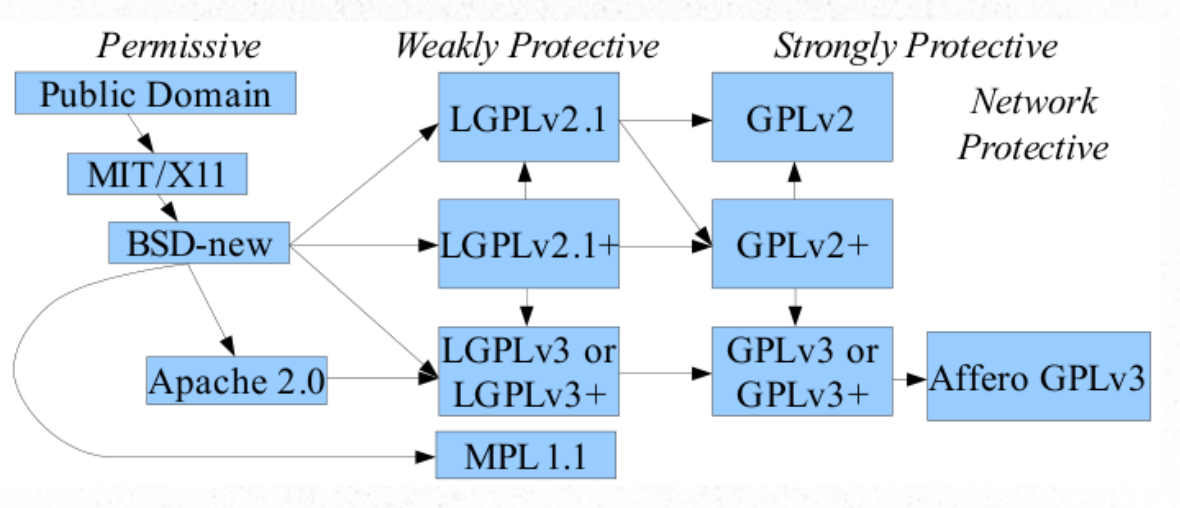
\includegraphics[width=100mm]{images/license-compatibility.png}
\caption{Mappa di compatibilità delle licenze}
\end{figure}
\section{Open Content}

\subsection*{Materiale di riferimento}

\begin{itemize}

\item \textbf{Viral Spiral, How the Commoners Built a Digital Republic of Their Own} - David Bollier;
\item La licenza GFDL \url{https://it.wikipedia.org/wiki/GNU_Free_Documentation_License};
\item \textbf{Creative Commons: a user guide} - Simone Aliprandi.

\end{itemize}

\subsection{I primi tentativi}

La \textbf{GNU Free Documentation License} è partita all'inizio perchè c'era la necessità di avere una \textbf{documentazione libera}. Per molto tempo la documentazione che accompagnava il software libero era sotto licenza GPL e lo stesso TLDP (The Linux Documentation Project) distribuiva la sua documentazione sotto GPL, semplicemente perchè era quello che ``passava al convento'', ma non ha molto senso usare la GPL per della documentazione. Se per esempio i \textit{Promessi Sposi} fosstrasparentiero sotto licenza GPL io potrei prendere i sorgenti e cambiare nella copertina il nome dell'autore: questo posso farlo tranquillamente senza problemi se sono sotto GPL. Ma questo è un problema perchè c'è differenza tra protezione del software e protezione del contenuto testuale. La tutela dell'autore originale è importante. Per questo motivo la GNU Free DOcumentation License si è posta come obiettivo una documentazione che avesse:

\begin{itemize}

\item Libertà di modifica;
\item Tutele dei diritti morali dell'autore;
\item Gestione del problema legato alle copie non trasparenti; come nel caso della GPL si vuole far sì che se qualcuno modifica un prodotto che è sotto GFDL quello rimanga disponibile nei suoi sorgenti (ad esempio non posso redistribuire un documento come serie di immagini jpeg che non sono editabili) e che non limiti la libertà di terzi di modificare la documentazione;
\item Copia in grande quantità e non.

\end{itemize}

\subsection{Concetti fondamentali}

È una licenza che nasce per la \textbf{documentazione} (soprattutto del progetto GNU). Si sente la necessità di dare al prodotto la possibilità di avere una documentazione sempre aggiornata quando esso viene rilasciato. Se ad esempio attuo una modifica al programma è necessario modificare la documentazione che ci sta dietro. 

Le parti del documento da considerare sono:

\begin{itemize}

\item Il \textbf{titolo}; se io modifico un documento sotto GFDL devo mantenere l'autore originale nella copertina aggiungendo eventualmente il mio;
\item Il documento in sè e il suo \textbf{contenuto};
\item \textbf{Sezioni secondarie e invarianti}, come ad esempio le dediche che possono essere modificate solamente mantenendo inalterato il tono. Le sezioni invarianti non possono assolutamente essere modificate ma devono essere al di fuori dell'argomento principale del documento;
\item \textbf{Testi di copertina}; posso modificare la copertina ma devo dichiararmi editore di quella versione;
\item \textbf{Storia del documento}, devo tenere traccia di tutte le modifiche e scriverle in una sezione del documento (esempio sezione Diario delle Modifiche);
\item La \textbf{licenza} dev'essere mantenuta e riportata nel documento.

\end{itemize}

Per quanto riguarda le copie trasparenti ci sono distinzioni per chi distribuisce sotto piccola quantità e grande quantità. In particolare se io voglio pubblicare un documento sul mio sito devo renderlo accessibile. Inoltre non devo aggiungere delle \textbf{restrizioni tecnologiche} che impediscano la modifica. 

Esiste tutta una serie di restrizioni per quanto riguarda la redistribuzione di \textbf{copie senza modifiche}:

\begin{itemize}

\item Mantenimento della licenza;
\item Nessuna misura tecnologica di restrizione;
\item Permettere di esibire la copia in pubblico;
\item Per quanto riguarda le redistribuzioni voluminose:
	\begin{itemize}

	\item Obbligo di identificarsi come autore;
	\item Obbligo di mantenere titoli e testi di copertina;
	\item Obbligo di distribuire una sorgente trasparente.

	\end{itemize}

\end{itemize}

Per quanto riguarda la redistribuzione di \textbf{copie modificate}:

\begin{itemize}

\item Devo modificare il titolo, in questo modo identifico il mio prodotto come qualcosa di diverso;
\item Indicazione degli autori delle modifiche e del documento originale;
\item Rimozione e/o aggiunta dei ``riconoscimenti'';
\item Aggiornamento della sezione cronologia;
\item Preservazione degli invarianti;
\item Preservazione della versione trasparente;
\item Preservazione e/o aggiunta dei testi di copertina.

\end{itemize}

Esistono anche tutta una serie di paragrafi di questa licenza che parlano essenzialmente dell'\textbf{unione di documenti}, delle collezioni e aggregati e delle \textbf{traduzioni} dei documenti. Per quanto riguarda le unioni di più documenti è necessario:

\begin{itemize}

\item Disambiguare tutte le parti;
\item Mantenere una licenza;
\item Rimuovere i riconoscimenti.

\end{itemize}

Un caso particolare è quando si tratta delle traduzioni: la traduzione è comunque considerata una modifica e in questo caso è necessario conservare la licenza e allo stesso tempo conservare gli invarianti. In questo modo si da garanzia all'autore che la sua opera non possa venire mal interpretata perchè io potrei tradurla in maniera non appropriata (scritta male o con ambiguità). È possibile in ogni caso prendere accordi con l'autore.

\subsection{Il fallimento del copyright}

C'è stato un cambiamento enorme per quanto riguarda i tipi di diritti associati agli utenti e agli sviluppatori del software. 

\subsection{Gli anni d'oro della proprietà intellettuale}

\subsection{I primi cambiamenti}

\subsection{I prodromi della crisi}

\subsection{Il movimento degli accademici}

\subsection{Mickey Mouse Protection Art}

\subsection{Eldred vs Reno}

\subsection{Creative Common}

\subsection{Le licenze Creative Common}
%\include{rdf}
%\section{SVN}

\subsection*{Materiale di riferimento}

\begin{itemize}

\item \textbf{Version Control with Subversion} Rilasciato sotto licenza CC 
all'indirizzo:
 \url{http://svnbook.red-bean.com/};
\item \textbf{Introduzione a git} - Luca De Franceschi 

\url{https://prezi.com/ayb1s8iahdi3/introduzione-a-git}
 \item \textbf{Pro Git} \url{https://git-scm.com/book/it/v1/}
\item \textbf{Pragmatic Version Control using Subversion} - Mike Mason 

\url{https://asudev.jira.com/wiki/download/attachments/49419503/Pragmatic_Version_Control_using_Subversion.pdf}.

\end{itemize}

\subsection{Version Control System}
Il controllo di versione è un sistema che registra, nel tempo, i cambiamenti di uno o più file, così da poter richiamare una specifica versione in un secondo momento. Qualsiasi file di un computer può essere posto sotto controllo di versione.

Un Sistema per il Controllo di Versione (Version Control System - VCS)  permette di ripristinare i file ad una versione precedente, ripristinare l'intero progetto a uno stato precedente, revisionare le modifiche fatte nel tempo, vedere chi ha cambiato qualcosa che può aver causato un problema, chi ha introdotto un problema e quando, riprtistinare il tutto in caso di problemi e molto altro ancora. 

I sistemi di controllo di versione si dividono in varie tipologie: 
\begin{itemize}
\item \textbf{Locali} Molte persone gestiscono le diverse versioni copiando i file in un'altra directory, questo semplice approccio è semplice, ma soggetto a frequenti errori. 

I VCS locali hanno un database semplice che mantiene tutti i cambiamenti dei file sotto controllo di revisione. Uno dei più famosi VCS locali è rcs che  funziona salvando sul disco una serie di patch (ovvero le differenze tra i file) tra una versione e l'altra, in un formato specifico; può quindi ricreare lo stato di qualsiasi file in qualsiasi momento determinato momento, aggiungendo le varie patch.

\item \textbf{Centralizzati} Affrontano il problema del collaborare con altri sviluppatori su altri sistemi. \textit{Subversion (SVN)} e \textit{Perforce}, hanno un unico server che contiene tutte le versioni dei file e gli utenti scaricano i file dal server centrale. Questo è stato lo standard del controllo di versione per molti anni.

\textbf{Pro:} 
\begin{itemize}
\item Chiunque sa, cosa stia facendo un'altra persona del progetto. \item Gli amministratori hanno un controllo preciso sugli utenti
\end{itemize}

\textbf{Contro:} 
In caso il server sia offline non è possibile lavorare, se il server centrale viene danneggiato e non c'è backup si perde tutto.

\item \textbf{Distribuiti} Es. \textit{git}, \textit{Mercurial}, \textit{Bazaar}, \textit{Darcs}. I client locali non solo controllano lo snapshot (una panoramica completa dello stato del repository) più recente dei file, ma fanno una copia completa del repository. In questo modo se un server morisse il repository di un qualsiasi client può essere copiato sul server per ripristinarlo. Ogni checkout è un backup completo di tutti i dati.
\end{itemize}

\subsection{SVN: I primi passi}
\subsubsection{Terminologia}
\begin{itemize}
\item \textbf{Repository} E' dove i file sono memorizzati, spesso su un server o in locale. Talvolta è chiamato anche depot (ad esempio in Perforce). Un repository può contenere uno o più progetti.

\item \textbf{Working copy} La directory di lavoro locale.

\item \textbf{Commit}
Un commit (o, più raramente, submit) si effettua quando si copiano le modifiche fatte su file locali nella directory del repository (il software di controllo versione controlla quali file sono stati modificati dall'ultima sincronizzazione).

\item \textbf{Modifica}
Una modifica (change) rappresenta una specifica modifica ad un documento sottoposto al VCS. La granularità delle modifiche considerate come cambiamenti varia tra i sistemi di controllo versione.

\item \textbf{Change List}
Su molti sistemi di controllo versione con commit di modifiche multiple atomiche, una changelist identifica un insieme di changes fatti in un singolo commit.

\item \textbf{Checkout}
Un check-out (o checkout o co) effettua una copia di lavoro dal repository (può essere visto come l'operazione inversa dell'importazione).

\item \textbf{Update}
Un update (o sync) copia le modifiche fatte sul repository nella propria directory di lavoro (può essere visto come l'operazione inversa del commit).

\item \textbf{Merge}
Un merge o integrazione unisce modifiche concorrenti in una revisione unificata.

\item \textbf{Revisione}
Una revisione o versione è una versione in una catena di modifiche.

\item \textbf{Import}
Il termine import è usato per descrivere la copiatura dell'intero albero di directory locale sul repository.

\item \textbf{Export}
Un export è simile ad un check-out eccetto il fatto che crea un albero di directory vuoto senza metadati di controllo versione (spesso è usato precedentemente alla pubblicazione dei contenuti).

\item \textbf{Conflitto}
Un conflitto si presenta quando diversi soggetti fanno modifiche in contemporanea allo stesso documento non vedendo l'uno le modifiche che sta apportando l'altro e che potrebbero sovrapporsi. Non essendo il software abbastanza intelligente da decidere quale tra le modifiche è quella 'corretta', si richiede ad un utente di risolvere il conflitto.

\item \textbf{Risolvere}
L'intervento di un utente per la risoluzione di un conflitto tra modifiche differenti di uno stesso documento.
\end{itemize}

\subsubsection{Installare SVN}
E' possibile installare agevolmente SVN su tutti i sistemi operativi più diffusi:

\begin{itemize}
\item \textbf{Windows}: Il miglior pacchetto comprensivo di gui è TortoiseSVN scaricabile al link \url{http://tortoisesvn.net/downloads.html}
\item \textbf{Linux}: Basta aprire un terminale e dare il comando adatto 
\begin{itemize}
\item Ubuntu \textit{sudo apt-get install subversion} 
\item Fedora \textit{sudo dnf install subversion} 
\item openSUSE \textit{sudo zypper install subversion} 
\end{itemize}
\item Mac: \url{https://subversion.apache.org/packages.html#osx}
\end{itemize}

\subsection{Repositories}
\subsection{Locking}
\subsubsection{Il problema}
\subsubsection{La soluzione lock - modify - unlock}
\subsubsection{La soluzione copy - modify - merge}
\subsection{Struttura di un repository}
\subsection{Valori simbolici di revisione}
\subsection{Ciclo fondamentale}
\subsection{Revisioni miste}
\subsection{Popolazione del repository}
\subsection{Creazione di un repository}
\subsection{Manipolazione del repository manualmente}
\subsection{Changelist}
\subsection{Controllo delle proprie modifiche}
\subsection{Usiamo diff}
\subsection{Annulliamo le nostre modifiche}
\subsection{Branches}
\subsection{Tags}
\subsection{Esempi}

%\section{git}

%\appendix

%\section{Glossario}

\subsection*{A}

\underline{\textbf{ARPA}}: %TODO

\underline{\textbf{ARPANET}}: %TODO

\underline{\textbf{Assembler}}: %TODO

\subsection*{B}

\underline{\textbf{Beowulf}}: %TODO

\subsection*{C}

\subsection*{D}

\underline{\textbf{Debian}}: %TODO

\underline{\textbf{DFSG}}: %TODO

\subsection*{E}

\subsection*{F}

\underline{\textbf{Free Software Foundation}}: %TODO

\underline{\textbf{Freeware}}: %TODO

\underline{\textbf{fsf}}: %TODO

\subsection*{G}

\underline{\textbf{GNU}}: %TODO

\underline{\textbf{GPL}}: %TODO

\subsection*{H}

\subsection*{I}

\subsection*{J}

\subsection*{K}

\underline{\textbf{Kernel}}: %TODO

\subsection*{L}

\underline{\textbf{Linux}}: %TODO

\subsection*{M}

\underline{\textbf{Mimix}}: %TODO

\underline{\textbf{MUTIX}}: %TODO

\subsection*{N}

\underline{\textbf{Netscape}}: %TODO

\underline{\textbf{nslu2}}: %TODO

\subsection*{O}

\underline{\textbf{OSI}}: %TODO

\subsection*{P}

\underline{\textbf{PDP}}: %TODO

\subsection*{Q}

\subsection*{R}

\underline{\textbf{RedHat Enterprise Linux}}: %TODO

\underline{\textbf{Routes}}: %TODO



\subsection*{S}

\underline{\textbf{StarOffice}}: %TODO

\underline{\textbf{Sun}}: 

\underline{\textbf{S\&P}}: %TODO

\underline{\textbf{Shareware}}: %TODO

\underline{\textbf{Symbolics}}: %TODO	

\subsection*{T}

\underline{\textbf{TECO}}: %TODO

\subsection*{U}

\underline{\textbf{Unix}}: %TODO

\subsection*{V}

\subsection*{W}

\subsection*{X}

\subsection*{Y}

\subsection*{Z}


	






\end{document}